\documentclass[12pt,a4paper]{article}

% ---------- 编码与字体 ----------
\usepackage[UTF8]{ctex}
\usepackage{xspace}
\emergencystretch=3em

% ---------- 页面布局 ----------
\usepackage{geometry}
\geometry{a4paper, left=2.5cm, right=2.5cm, top=2.8cm, bottom=2.8cm}

% ---------- 颜色 ----------
\usepackage[table,dvipsnames,svgnames]{xcolor}
\definecolor{primary}{HTML}{1F3864}       % 深海军蓝：标题、链接
\definecolor{secondary}{HTML}{4A6B8A}     % 次要蓝灰
\definecolor{accent}{HTML}{2E74B5}        % 强调蓝
\definecolor{lightbg}{HTML}{F5F6F8}       % 代码块浅灰底
\definecolor{darkgray}{HTML}{333333}
\definecolor{infocolor}{RGB}{46,116,181}  % 信息框：蓝
\definecolor{tipcolor}{RGB}{63,140,63}    % 提示框：绿
\definecolor{warncolor}{RGB}{214,138,40}  % 注意框：琥珀
\definecolor{dangercolor}{RGB}{200,60,60} % 危险框：红

% ---------- 图形 ----------
\usepackage{graphicx}
\usepackage{subcaption}
\usepackage{tikz}
\usetikzlibrary{
    shapes.geometric, arrows.meta, positioning,
    backgrounds, shadows.blur, calc
}

% ---------- 数学 ----------
\usepackage{amsmath, amssymb}
\usepackage{mathtools}

% ---------- 表格与代码 ----------
\usepackage{array, booktabs, multirow, longtable, makecell}
\usepackage{seqsplit}
\usepackage{listings}
\lstset{
    basicstyle=\small\ttfamily,
    numbers=left,
    numberstyle=\tiny\color{gray},
    frame=single,
    rulecolor=\color{gray!50},
    backgroundcolor=\color{lightbg},
    breaklines=true,
    keywordstyle=\color{primary}\bfseries,
    commentstyle=\color{gray}\itshape,
    stringstyle=\color{secondary},
    showstringspaces=false,
    captionpos=b,
    xleftmargin=2em,
    xrightmargin=1em,
    aboveskip=1em,
    belowskip=1em,
}

% ---------- 页眉页脚 ----------
\usepackage{fancyhdr}
\usepackage{lastpage}
\pagestyle{fancy}
\setlength{\headheight}{22pt}
\fancyhf{}
\fancyhead[L]{\color{darkgray}\small\heiti PendulumLab 倒立摆实验设备使用指南}
\fancyhead[R]{\color{darkgray}\small 第\,\thepage\,页\ / 共\,\pageref{LastPage}\,页}
\fancyfoot[C]{\color{gray}\tiny PendulumLab 实验平台 · 文档版本 V2.0 · \the\year}
\renewcommand{\headrulewidth}{0.4pt}
\renewcommand{\headrule}{\hbox to\headwidth{\color{gray!60}\leaders\hrule height \headrulewidth\hfill}}

% ---------- 章节、列表与盒子 ----------
\usepackage{titlesec}
\titleformat{\section}[hang]
    {\LARGE\heiti\bfseries}
    {\thesection\enspace}
    {0pt}
    {}
    [\vspace{-0.6em}{\color{gray!50}\rule{\textwidth}{0.7pt}}]
\titleformat{\subsection}[hang]
    {\Large\heiti\color{primary}}
    {\thesubsection\enspace}
    {0pt}
    {}
\titleformat{\subsubsection}[hang]
    {\large\heiti\color{darkgray}}
    {\thesubsubsection\enspace}
    {0pt}
    {}

\usepackage{enumitem}
\setlist{nosep, leftmargin=*}
\setlist[itemize]{label=\textbullet}
\setlist[enumerate]{label=\arabic*.}

\usepackage[most]{tcolorbox}
\tcbset{
    enhanced,
    frame hidden,
    boxrule=0pt,
    fonttitle=\heiti\bfseries,
    boxsep=4pt,
    left=10pt,
    right=8pt,
    top=8pt,
    bottom=8pt,
    arc=2pt,
    toptitle=2pt,
    bottomtitle=2pt,
}
\newtcolorbox{infobox}{
    borderline west={3pt}{0pt}{infocolor},
    colback=infocolor!6,
    coltitle=infocolor!65!black,
    title=信息,
}
\newtcolorbox{tipbox}{
    borderline west={3pt}{0pt}{tipcolor},
    colback=tipcolor!6,
    coltitle=tipcolor!65!black,
    title=提示,
}
\newtcolorbox{warnbox}{
    borderline west={3pt}{0pt}{warncolor},
    colback=warncolor!7,
    coltitle=warncolor!65!black,
    title=注意,
}
\newtcolorbox{dangerbox}{
    borderline west={3pt}{0pt}{dangercolor},
    colback=dangercolor!6,
    coltitle=dangercolor!70!black,
    title=危险,
}

% ---------- 超链接与算法 ----------
\usepackage{hyperref}
\hypersetup{
    colorlinks=true,
    linkcolor=accent,
    urlcolor=accent,
    citecolor=accent,
    pdftitle={PendulumLab 倒立摆实验设备使用指南},
    pdfauthor={PendulumLab 实验平台},
}
\usepackage{algorithm}
\usepackage{algpseudocode}
\usepackage{pifont}
\newcommand{\cmark}{\ding{51}}
\newcommand{\xmark}{\ding{55}}

% ---------- 自定命令 ----------
\newcommand{\latex}{\LaTeX\xspace}

\begin{document}

% ======================================================================
\begin{titlepage}
    \centering
    \vspace*{1.5cm}
    {\color{gray}\heiti PendulumLab 实验平台}\\[0.8em]
    {\color{gray!60}\rule{0.72\textwidth}{0.4pt}}\\[2.2em]

    {\fontsize{28pt}{40pt}\selectfont\heiti 倒立摆实验设备使用指南}\\[1em]
    {\Large\heiti PendulumLab 一级 / 二级倒立摆}\\[0.5em]
    {\Large 使用与算法开发手册}\\[0.7em]
    {\normalsize\color{gray} Usage Guide \& Development Manual}\\[2.6em]

    {\heiti 文档信息}\\[0.6em]
    \begin{tabular}{@{}>{\heiti\small}p{3.2cm} p{9.6cm}@{}}
        \toprule
        文档编号 & PL-UM-2026-001 \\
        文档版本 & V2.0 \\
        编制日期 & \today \\
        适用型号 & 一级倒立摆（\texttt{Pendulum\_Native\_1.slx}）\\
                 & 二级倒立摆（\texttt{Pendulum\_Native\_2.slx}）\\
        适用范围 & 首次接触设备的学生、教师与算法工程师 \\
        文档状态 & 发布 \\
        \bottomrule
    \end{tabular}\\[2.4em]

    {\heiti 修订记录}\\[0.6em]
    \begin{tabular}{@{}cccc@{}}
        \toprule
        \textbf{版本} & \textbf{日期} & \textbf{修订说明} & \textbf{修订人} \\
        \midrule
        V1.0 & 2026-09-08 & 首次发布 & --- \\
        \bottomrule
    \end{tabular}

    \vfill
    {\color{gray!60}\rule{0.72\textwidth}{0.4pt}}\\[1.2em]
    {\small\color{gray} 编制单位：PendulumLab 实验平台}\\[0.4em]
    {\small\color{gray} \copyright\ \the\year\ · 本文档仅供平台用户内部使用}
\end{titlepage}

\newpage
\begin{dangerbox}
    \textbf{重启安全强制要求：}在重启电脑、MATLAB、Simulink、数据采集设备、伺服驱动器或倒立摆系统中的任何设备之前，必须先按下急停按钮；重启完成后也必须保持急停按钮处于按下状态。只有完成人员确认、轨道清障、限位检查、通信检查和只读预检后，才允许由现场操作人员解除急停。不得依赖软件 Stop、程序退出或电脑关机代替急停。
\end{dangerbox}

\begin{warnbox}
    任何异常重启、断电恢复、驱动器报警复位或程序崩溃，都按“重新上电”处理：先确认急停已按下，再进行恢复操作。
\end{warnbox}

\newpage
\pagenumbering{Roman}
\setcounter{tocdepth}{2}
{\hypersetup{linkcolor=accent}\tableofcontents}
\newpage
\pagenumbering{arabic}

% ======================================================================
\section{引言与使用须知}
\label{sec:intro}

本指南介绍 PendulumLab 一级 / 二级倒立摆实验平台的完整使用方法，内容整合自平台配套的《Simulink 算法开发与使用指南》与《MATLAB 离线仿真与 LQR 算法指南》。倒立摆是控制理论教学与科研中最经典的实验对象之一：系统本身不稳定、非线性强、对实时性要求高，非常适合用来验证摆起控制（Swing-up）、LQR 稳定控制、状态估计与嵌入式实时控制等内容。

\begin{infobox}
    平台已经封装好硬件采集、执行器输出、自动回中、零点采集、实时节拍、数据记录和安全停机。\textbf{算法使用者只需要修改 Simulink 模型中的 \texttt{Control} 子系统}，不需要重新连接或编写硬件输入输出。
\end{infobox}

各章节内容与适用读者如下：

\begin{center}
    \renewcommand{\arraystretch}{1.4}
    \begin{tabular}{@{}c p{8.9cm} c@{}}
        \toprule
        \textbf{章节} & \textbf{内容} & \textbf{适用读者} \\
        \midrule
        第~\ref{sec:overview} 节 & 设备组成、型号参数与系统架构 & 首次接触设备 \\
        第~\ref{sec:quickstart} 节 & 五分钟快速上手工作流 & 所有读者 \\
        第~\ref{sec:simulink} 节 & Simulink 实机模型与固定接口 & 算法开发人员 \\
        第~\ref{sec:matlab} 节 & MATLAB 离线仿真与验证 & 算法开发人员 \\
        第~\ref{sec:algorithm} 节 & 摆起与 LQR 控制算法原理 & 所有读者 \\
        第~\ref{sec:migration} 节 & 从离线仿真迁移到实机 & 算法开发人员 \\
        第~\ref{sec:hardware} 节 & 实机运行操作流程 & 所有读者 \\
        第~\ref{sec:safety} 节 & 安全规范与禁止修改区域 & \textbf{必读} \\
        第~\ref{sec:faq} 节 & 常见问题排查 & 所有读者 \\
        附录 & 命令速查与文件地图 & 所有读者 \\
        \bottomrule
    \end{tabular}
\end{center}

\begin{warnbox}
    \textbf{使用须知：} 首次接触设备的用户，请先通读第~\ref{sec:overview} 节（设备概述）、第~\ref{sec:quickstart} 节（快速上手）和第~\ref{sec:safety} 节（安全规范）。首次实机运行必须有人值守，并采用有限运行时间（见第~\ref{sec:hardware} 节）。
\end{warnbox}

% ======================================================================
\section{设备概述}
\label{sec:overview}

\subsection{平台组成}

PendulumLab 倒立摆实验平台由机械部分、电气部分和上位机软件三部分组成：

\begin{itemize}
    \item \textbf{机械部分}：直线轨道、可在轨道上自由滑动的小车、可绕关节自由旋转的摆杆（一级摆为 1 根摆杆，二级摆为 2 根摆杆串联）、转轴与关节编码器。
    \item \textbf{电气部分}：伺服电机与安川 SGD7S 系列驱动器、小车与摆杆的增量式编码器、左右物理限位开关、急停装置、NI PCI-6602 计数器板卡和 Advantech PCI-1723 模拟量输出板卡。
    \item \textbf{软件部分}：MATLAB + Simulink 环境，包含实机控制模型与离线仿真模型两套体系。
\end{itemize}

\begin{tipbox}
    设备外观、接线、铭牌与开关布局以实物和随箱说明为准。本指南重点覆盖软件操作、算法开发与安全规范；软件层的接口定义对设备操作至关重要，请重点关注第~\ref{sec:simulink} 节。
\end{tipbox}

\subsection{两个型号}

平台提供一级摆与二级摆两个型号，对应两个 Simulink 实机模型：

\begin{center}
    \renewcommand{\arraystretch}{1.4}
    \begin{tabular}{@{}lcccl@{}}
        \toprule
        \textbf{型号} & \textbf{实机模型} & \textbf{采样周期} & \textbf{控制频率} & \textbf{状态数} \\
        \midrule
        一级倒立摆 & \texttt{Pendulum\_Native\_1.slx} & 0.01\,s & 100\,Hz & 4 \\
        二级倒立摆 & \texttt{Pendulum\_Native\_2.slx} & 0.005\,s & 200\,Hz & 6 \\
        \bottomrule
    \end{tabular}
\end{center}

二级摆与一级摆相比，增加了一根摆杆及其编码器，控制频率翻倍、状态数由 4 变为 6，控制难度显著提高。

\subsection{实机硬件与通道参数}

表中参数来自当前项目的 \texttt{ph\_config.m} 和 \texttt{config/config.json}。更换板卡、驱动器、接线或编码器后，必须重新核对配置，不能直接沿用。

\begin{longtable}{@{}p{4.2cm} p{4.4cm} p{6.0cm}@{}}
    \caption{实机硬件与通道参数}\label{tab:hardwareparams}\\
    \toprule
    \textbf{项目} & \textbf{当前值} & \textbf{说明} \\
    \midrule
    \endfirsthead
    \toprule
    \textbf{项目} & \textbf{当前值} & \textbf{说明} \\
    \midrule
    \endhead
    \bottomrule
    \endlastfoot
    计数器板卡 & NI PCI-6602，\texttt{Dev1} & 读取编码器和数字限位 \\
    模拟量输出板卡 & PCI-1723，\texttt{BID\#15} & AO0 输出控制电压 \\
    伺服驱动器 & SGD7S-180A00A002 & 模拟速度控制模式 \\
    小车编码器 & \texttt{Dev1/ctr0} & X4 解码；当前按 8000 count/rev 配置 \\
    一级摆编码器 & \texttt{Dev1/ctr1} & X4 解码；8000 count/rev \\
    二级摆编码器 & \texttt{Dev1/ctr2} & X4 解码；4000 count/rev \\
    编码器数字滤波 & $10\,\mu\text{s}$ & 最小有效脉宽 \\
    左限位 & \texttt{Dev1/port0/line0} & 高电平有效 \\
    右限位 & \texttt{Dev1/port0/line2} & 高电平有效 \\
    伺服使能 & \texttt{Dev1/port0/line3} & 高电平有效 \\
    模拟量输出 & PCI-1723 AO0 & 正电压小车向右，负电压小车向左 \\
    板卡量程 & $-10\sim 10$ V & PCI-1723 配置范围，不是控制算法允许范围 \\
    控制电压限幅 & $-1\sim 1$ V & 正常摆起与稳摆的算法硬限幅 \\
    安全输出 & 0 V & 故障或停止时的目标输出 \\
    标定静止电压 & $-0.00152587890625$ V & 当前电机零速补偿值 \\
\end{longtable}

\subsection{采样、行程与启动参数}

\begin{table}[htbp]
    \centering
    \caption{一级与二级实机关键参数}
    \label{tab:runtimeparams}
    \renewcommand{\arraystretch}{1.35}
    \begin{tabular}{@{}p{5.8cm}cc@{}}
        \toprule
        \textbf{参数} & \textbf{一级摆} & \textbf{二级摆} \\
        \midrule
        控制周期 & 0.01 s & 0.005 s \\
        控制频率 & 100 Hz & 200 Hz \\
        采样超时 & 0.05 s & 0.05 s \\
        小车位置换算 & $0.163/8000$ m/count & $0.734/33259$ m/count \\
        软件预警位置 & 0.25 m & 0.30 m \\
        软件停止位置 & 0.30 m & 0.35 m \\
        加速度限幅 & $\pm10$ m/s$^2$ & $\pm30$ m/s$^2$ \\
        下垂零点采集时间 & 1.5 s & 1.5 s \\
        零点等待超时 & 20 s & 30 s \\
        一级摆零点最大跨度 & 8 count & 80 count \\
        二级摆零点最大跨度 & --- & 40 count \\
        回中搜索电压 & \multicolumn{2}{c}{0.20 V} \\
        回中精搜索电压 & \multicolumn{2}{c}{0.02 V} \\
        限位释放电压 & \multicolumn{2}{c}{0.03 V} \\
        回中搜索超时 & \multicolumn{2}{c}{60 s} \\
        默认有限运行时间 & \multicolumn{2}{c}{60 s} \\
        \bottomrule
    \end{tabular}
\end{table}

\begin{warnbox}
    “板卡量程 $\pm10$ V”和“算法限幅 $\pm1$ V”含义不同。普通算法开发不得把控制限幅提高到板卡量程，也不得修改机械行程、限位极性或伺服使能极性。
\end{warnbox}

\subsection{离线物理模型参数}

\begin{table}[htbp]
    \centering
    \caption{一级摆离线物理与控制参数}
    \label{tab:singlephysical}
    \renewcommand{\arraystretch}{1.3}
    \begin{tabular}{@{}p{5.8cm}p{4.0cm}p{4.5cm}@{}}
        \toprule
        \textbf{参数} & \textbf{当前值} & \textbf{来源/含义} \\
        \midrule
        摆杆质量 $m$ & 0.134 kg & 参考模型参数 \\
        等效长度 $l$ & 0.2285 m & 参考模型参数 \\
        重力加速度 $g$ & 9.8 m/s$^2$ & 模型设定 \\
        关节转动惯量 $J$ & $\frac{4}{3}ml^2$ & 由参考模型关系推得 \\
        数值仿真步长 & 0.001 s & 固定步长 \\
        仿真时间 & 50 s & 标准验证场景 \\
        小车位置限制 & 0.35 m & 离线终止边界 \\
        摆起能量增益 & 5 & 能量控制参数 \\
        摆起速度限制 & 0.30 m/s & 轨道保护 \\
        LQR 捕获角度 & $\pi/6$ rad & 直立邻域 \\
        LQR 捕获角速度 & 3 rad/s & 切换条件 \\
        \bottomrule
    \end{tabular}
\end{table}

\begin{table}[htbp]
    \centering
    \caption{二级摆离线物理参数}
    \label{tab:doublephysical}
    \renewcommand{\arraystretch}{1.3}
    \begin{tabular}{@{}p{5.8cm}p{4.0cm}p{4.5cm}@{}}
        \toprule
        \textbf{参数} & \textbf{当前值} & \textbf{来源/含义} \\
        \midrule
        一级杆质量 $m_1$ & 0.3534 kg & 当前装置参数 \\
        二级杆质量 $m_2$ & 0.1016 kg & 当前装置参数 \\
        一级关节惯量 $J_1$ & 0.005160863235 kg$\cdot$m$^2$ & 物理摆测试修正均值 \\
        二级关节惯量 $J_2$ & 0.007028721867 kg$\cdot$m$^2$ & 细杆惯量及平行轴定理 \\
        一级质心距离 $l_1$ & 0.12 m & 当前装置参数 \\
        二级质心距离 $l_2$ & 0.23 m & 当前装置参数 \\
        一级杆几何长度 $L_1$ & 0.1294 m & 当前装置参数 \\
        二级杆几何长度 $L_2$ & 0.442 m & 当前装置参数 \\
        重力加速度 $g$ & 9.81 m/s$^2$ & 模型设定 \\
        数值仿真步长 & 0.001 s & 标准摆起验证 \\
        仿真时间 & 50 s & 标准摆起场景 \\
        \bottomrule
    \end{tabular}
\end{table}

\begin{infobox}
    离线物理参数用于算法验证，不等同于硬件驱动参数。质量、尺寸、惯量或机械结构发生变化后，应重新辨识模型、线性化并验证 LQR，不应只修改一个增益。
\end{infobox}

\subsection{两套软件体系}

\begin{center}
    \renewcommand{\arraystretch}{1.4}
    \begin{tabular}{@{}l p{7.8cm} c@{}}
        \toprule
        \textbf{体系} & \textbf{用途} & \textbf{是否驱动实机} \\
        \midrule
        \texttt{matlab/single\_pendulum} & 一级摆动力学、摆起和稳摆离线仿真 & 否 \\
        \texttt{matlab/double\_pendulum} & 二级摆动力学、三级摆起、LQR 设计和优化 & 否 \\
        \texttt{matlab/native\_simulink} & 连接真实硬件的控制图 & 是 \\
        \bottomrule
    \end{tabular}
\end{center}

离线系统和实机系统职责不同：\textbf{离线模型不连接真实板卡}，用于在修改实机 \texttt{Control} 之前验证算法。两套体系之间通过第~\ref{sec:migration} 节的迁移流程衔接。

\subsection{顶层架构与数据流}

实机 Simulink 模型的顶层由四个模块组成，数据流如图~\ref{fig:dataflow} 所示：

\begin{figure}[htbp]
    \centering
    \begin{tikzpicture}[
            node distance=1.7cm,
            block/.style={rectangle, draw=primary, line width=0.8pt, fill=primary!5, text width=8em, text centered, rounded corners=3pt, minimum height=2.8em, font=\small\bfseries},
            auxblock/.style={rectangle, draw=gray!60, fill=gray!6, text width=8em, text centered, rounded corners=3pt, minimum height=2.2em, font=\small},
            arrow/.style={-{Stealth}, thick, color=primary}
        ]
        \node [block] (hw) {Hardware};
        \node [block, right=3.0cm of hw] (nc) {Control};
        \node [auxblock, below=1.6cm of nc] (sync) {Real-Time Sync\\ 100/200\,Hz};
        \draw [arrow] (hw) -- node[above, font=\footnotesize]{角度、位置、限位、使能} (nc);
        \draw [arrow] (nc.north) to[out=90, in=90] node[above, font=\footnotesize]{加速度指令} (hw.north);
        \draw [-{Stealth}, thick, dashed, color=gray!70] (sync.west) -| (hw.south);
    \end{tikzpicture}
    \caption{PendulumLab 实机模型顶层数据流}
    \label{fig:dataflow}
\end{figure}

\begin{itemize}
    \item \texttt{Hardware} 负责读取编码器和限位、物理量换算、自动使能、加速度到电压、记录和安全停机；
    \item \texttt{Control} 是算法使用者唯一允许修改的模块，只输出加速度；
    \item \texttt{Real-Time Sync} 让模型在 Normal 模式下按 100\,Hz（一级）或 200\,Hz（二级）的真实时间节拍运行。
\end{itemize}

% ======================================================================
\section{快速上手：五分钟工作流}
\label{sec:quickstart}

\subsection{典型工作流}

\begin{dangerbox}
    开始任何操作前先确认急停状态。电脑、MATLAB、Simulink、板卡、伺服驱动器或设备任一部分发生重启时，必须立即按下并保持急停，完成全部重新检查后才能解除。
\end{dangerbox}

\begin{enumerate}
    \item 在 MATLAB/Simulink 中打开一级或二级实机模型（\texttt{matlab/native\_simulink/} 下的 \texttt{.slx} 文件）。
    \item 双击 \texttt{Control} 子系统进入其内部。
    \item 在子系统内部修改算法、增益、滤波器或状态切换逻辑。
    \item 保存 \texttt{.slx} 模型。
    \item 先运行离线一致性和故障测试（第~\ref{sec:matlab} 节、第~\ref{sec:hardware} 节）。
    \item 确认设备、限位和急停可用后再进行实机运行（第~\ref{sec:hardware} 节）。
    \item 点击 Simulink Stop 或按 \texttt{Ctrl+C} 停止运行，硬件层会自动关闭输出。
\end{enumerate}

\subsection{核心规则}

\begin{infobox}
    \textbf{核心规则：只修改 \texttt{Control} 内部。}
    不修改 \texttt{Hardware}、\texttt{Real-Time Sync}、顶层反馈线，以及 \texttt{Control} 的五个输入端口和一个输出端口。
\end{infobox}

\begin{warnbox}
    \textbf{不要运行 \texttt{pn\_build}。} 该脚本会从生成代码重建模型，可能覆盖你在 \texttt{.slx} 中保存的算法修改；只有需要恢复项目提供的原始控制器时才运行它。
    \texttt{pn\_verify()} 默认验证当前保存的模型而不重建；只有明确执行 \texttt{pn\_verify(true)} 或 \texttt{pn\_build()} 才会覆盖模型。
\end{warnbox}

% ======================================================================
\section{Simulink 实机模型与固定接口}
\label{sec:simulink}

\subsection{顶层模型}

一级摆与二级摆的顶层模型分别如图~\ref{fig:order1_top} 与图~\ref{fig:order2_top} 所示。两者采用相同的物理量接口；一级控制周期为 10\,ms，二级为 5\,ms。

\begin{figure}[htbp]
    \centering
    \begin{subfigure}{0.49\textwidth}
        \centering
        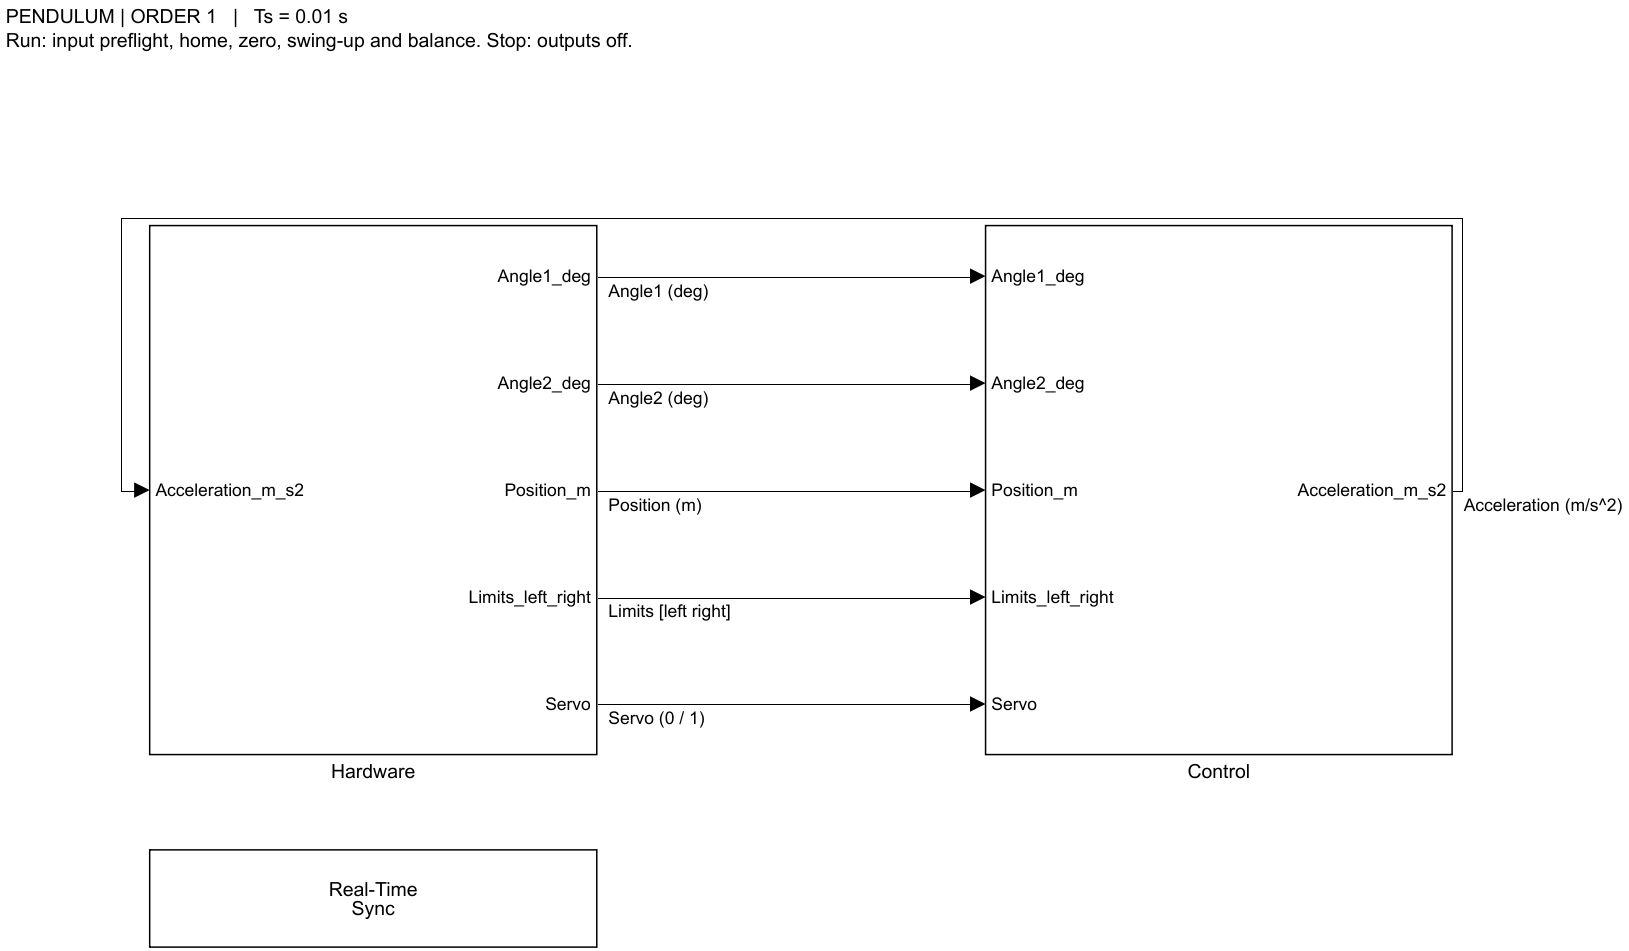
\includegraphics[width=\textwidth]{docs/simulink_algorithm_guide_assets/order1_top.png}
        \caption{一级摆顶层模型}
        \label{fig:order1_top}
    \end{subfigure}
    \hfill
    \begin{subfigure}{0.49\textwidth}
        \centering
        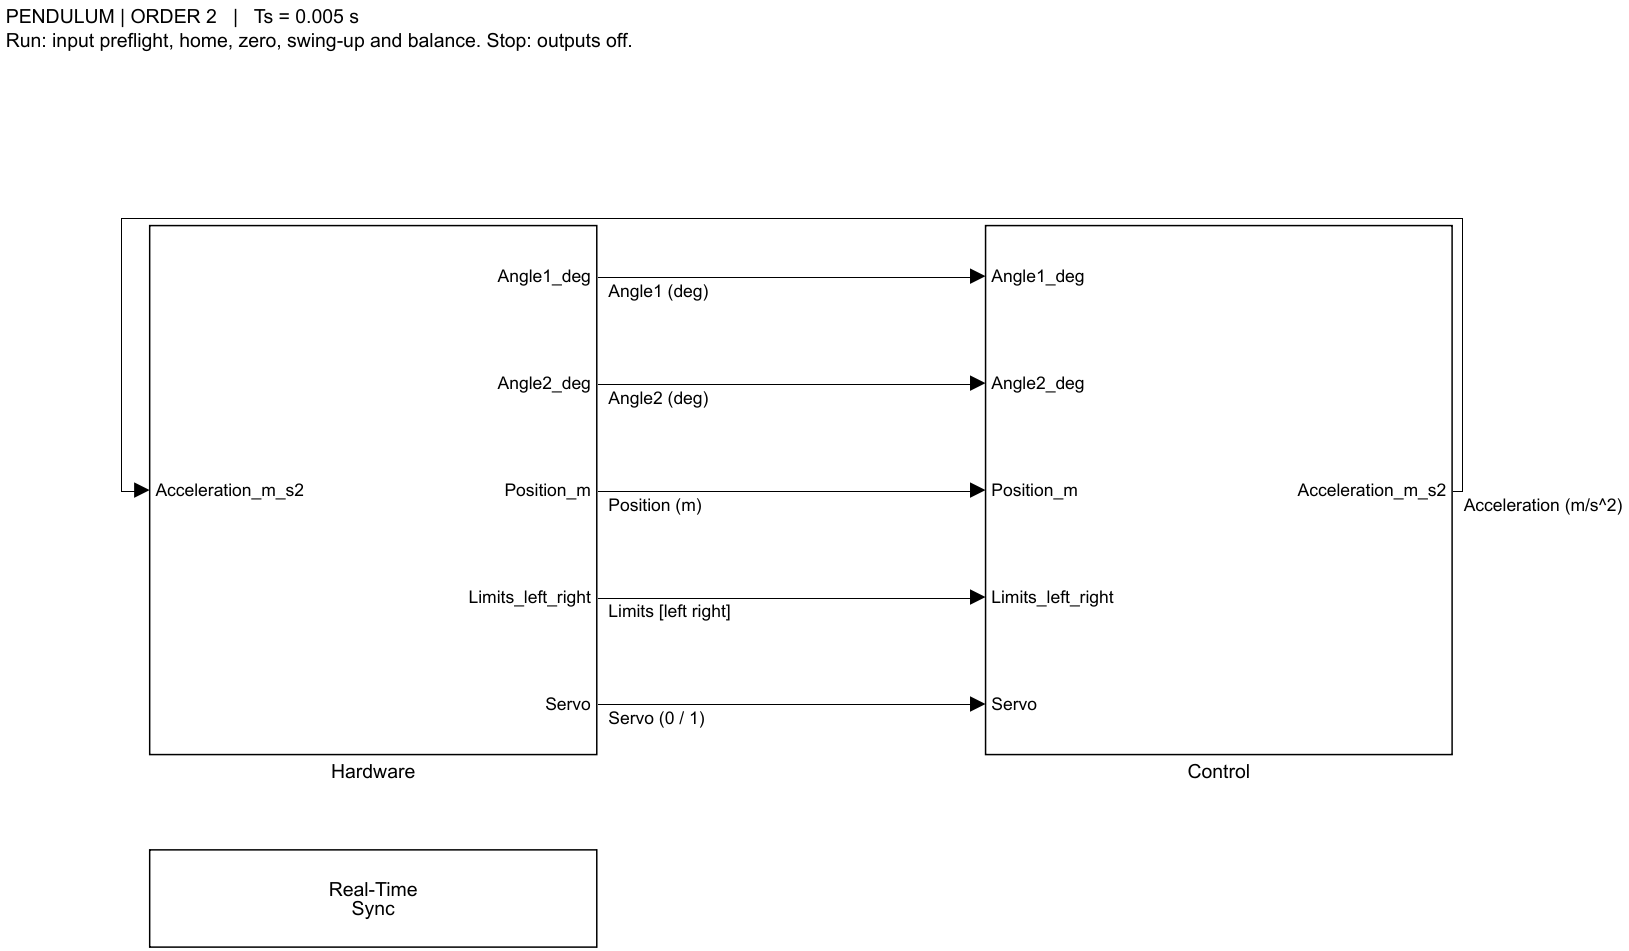
\includegraphics[width=\textwidth]{docs/simulink_algorithm_guide_assets/order2_top.png}
        \caption{二级摆顶层模型}
        \label{fig:order2_top}
    \end{subfigure}
    \caption{实机 Simulink 顶层模型}
\end{figure}

顶层各模块的职责与修改权限如下：

\begin{center}
    \renewcommand{\arraystretch}{1.4}
    \begin{tabular}{@{}l c p{9.4cm}@{}}
        \toprule
        \textbf{模块} & \textbf{可否修改} & \textbf{作用} \\
        \midrule
        \texttt{Hardware} & 否 & 回中标零、传感器换算、自动使能、加速度到电压、限位保护、记录与停机 \\
        \texttt{Control} & \textbf{是} & 状态估计、摆起、稳摆与阶段切换，只产生加速度指令 \\
        \texttt{Real-Time Sync} & 否 & 让 Normal 模式按照 100/200\,Hz 的真实时间节拍运行 \\
        \bottomrule
    \end{tabular}
\end{center}

\subsection{\texorpdfstring{\texttt{Control}}{Control} 的固定接口}

\texttt{Control} 固定为 5 个输入端口和 1 个输出端口。接口是算法与硬件之间唯一的约定，修改算法时必须保持端口顺序、维度、单位和符号不变。

\subsubsection{输入端口}

\begin{center}
    \renewcommand{\arraystretch}{1.4}
    \begin{tabular}{@{}c l l p{7.5cm}@{}}
        \toprule
        \textbf{端口} & \textbf{名称} & \textbf{维度} & \textbf{含义} \\
        \midrule
        1 & \texttt{Angle1\_deg} & 标量 & 第一杆绝对角，直立为 $0^\circ$，约在 $[-180^\circ,180^\circ]$ \\
        2 & \texttt{Angle2\_deg} & 标量 & 第二杆绝对角；一级模型固定为 0 \\
        3 & \texttt{Position\_m} & 标量 & 回中位置为 0，向右为正、向左为负，单位 m \\
        4 & \texttt{Limits\_left\_right} & 2 & $[\text{左},\text{右}]$；1 已触发、0 未触发 \\
        5 & \texttt{Servo} & 标量 & 启动流程自动产生的使能命令状态；1 开启、0 关闭 \\
        \bottomrule
    \end{tabular}
\end{center}

\begin{warnbox}
    \texttt{Servo} 表示程序发出的使能状态，不是驱动器独立反馈。使能仍由启动流程自动控制，算法不得通过该输入自行切换伺服。
\end{warnbox}

\subsubsection{输出端口}

唯一输出为 \texttt{Acceleration\_m\_s2}，是与位置正方向一致的标量加速度，单位 m/s$^2$。硬件层再次执行一级 $\pm10$、二级 $\pm30$ m/s$^2$ 限幅，并完成速度参考积分、PI 速度环、电压限幅和故障处理。

\begin{table}[htbp]
    \centering
    \caption{二级摆阶段切换与执行器控制参数}
    \label{tab:doublecontrolparams}
    \renewcommand{\arraystretch}{1.3}
    \begin{tabular}{@{}p{7.0cm}p{3.3cm}p{3.5cm}@{}}
        \toprule
        \textbf{参数} & \textbf{当前值} & \textbf{作用} \\
        \midrule
        速度滤波截止频率 & 20 Hz & 状态速度估计 \\
        速度参考限幅 & 0.6 m/s & 加速度积分限幅 \\
        速度环 $K_p$ & 0.18 & 速度误差比例项 \\
        速度环 $K_i$ & 54 & 速度误差积分项 \\
        Stage 1 捕获角 & 0.37 rad & 进入 Stage 2 \\
        Stage 1 回退角 & 0.70 rad & 回到 Stage 1 \\
        Stage 1 捕获角速度 & 2.0 rad/s & 切换约束 \\
        Stage 1 分段增益 & 2.1876 / 4.9156 / 8.2100 & 一级杆摆起 \\
        Stage 2 远区阈值 & 1.146 rad & 第二杆控制分区 \\
        Stage 2 远区/近区增益 & 1.40 / 5.00 & 第二杆能量控制 \\
        第二杆目标能量 & 0.005 J & 近区能量误差 \\
        Stage 3 捕获角 & 0.12 / 0.26 rad & 一级杆/二级杆 \\
        Stage 3 捕获角速度 & 0.60 / 0.80 rad/s & 一级杆/二级杆 \\
        捕获小车速度 & 0.12 m/s & Stage 3 切换约束 \\
        轨道软制动位置 & 0.22 m & 摆起阶段提前制动 \\
        轨道恢复位置 & 0.30 m & 实机向中心恢复 \\
        恢复电压 & 0.03 V & 二级软件行程恢复 \\
        \bottomrule
    \end{tabular}
\end{table}

\subsection{一级摆算法模块}

一级摆的 \texttt{Control} 内部只包含状态估计、摆起和稳摆算法；执行器内环与安全保护位于 \texttt{Hardware}。

\subsubsection{\texorpdfstring{\texttt{Sensor\_and\_memory}}{Sensor and memory}}

\begin{figure}[htbp]
    \centering
    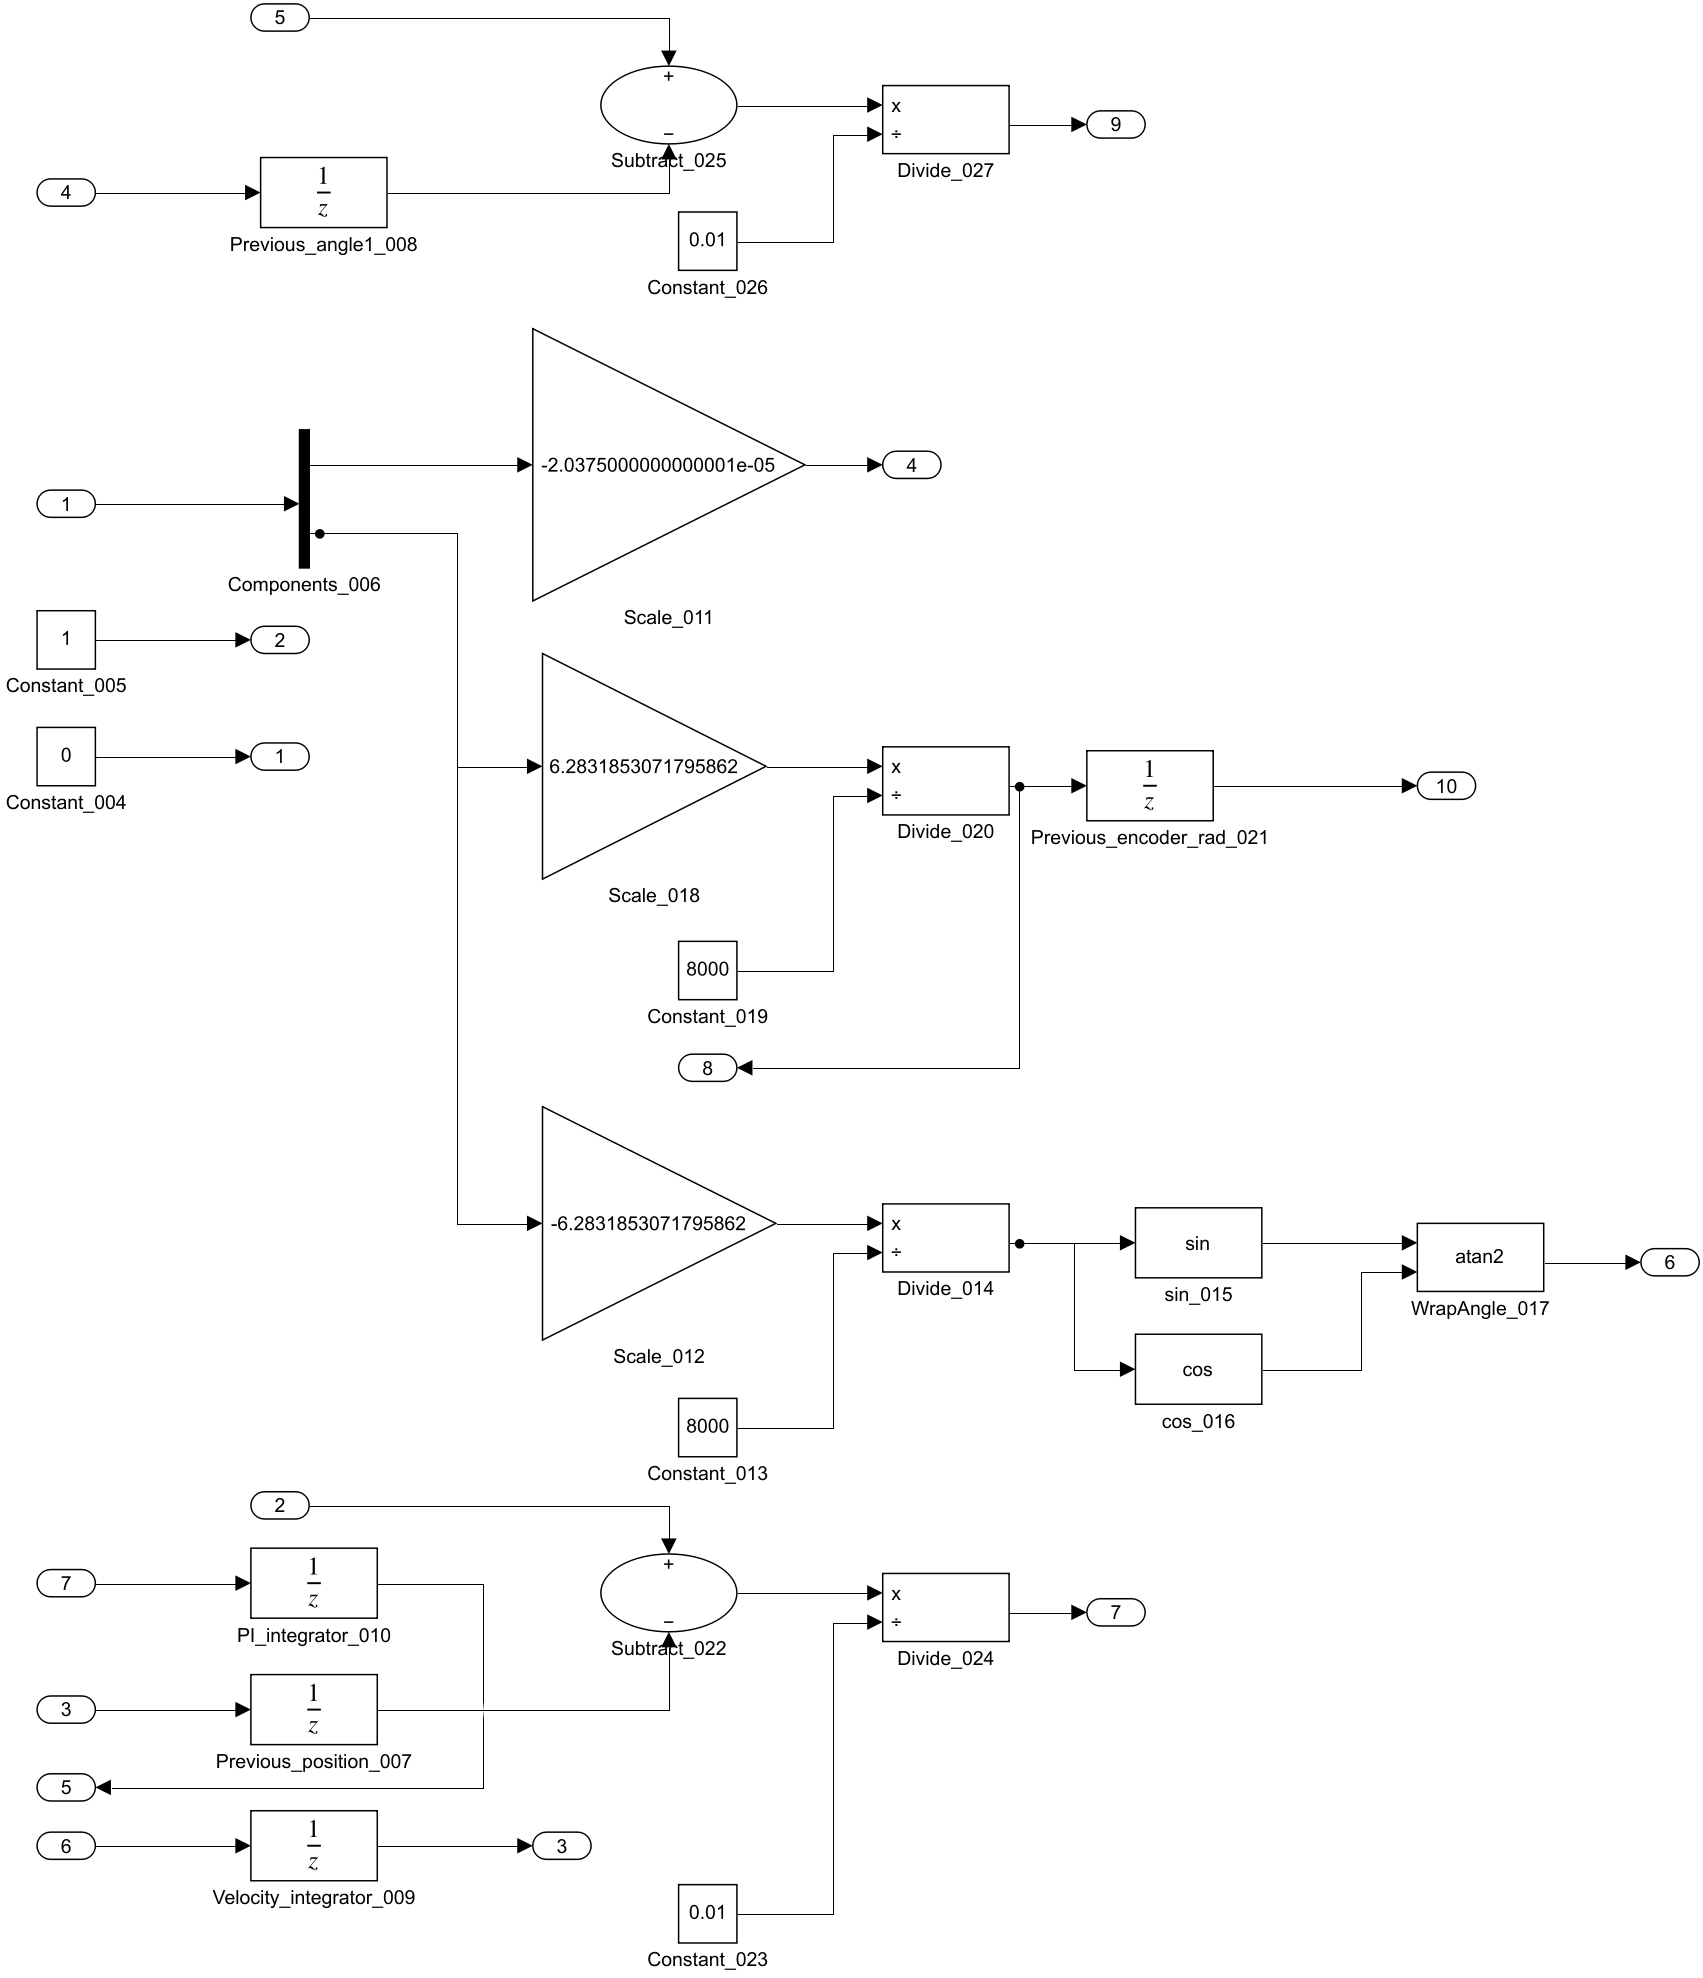
\includegraphics[width=0.55\textwidth]{docs/simulink_algorithm_guide_assets/order1_sensor_and_memory.png}
    \caption{一级摆：传感器与状态记忆模块}
    \label{fig:o1_sensor}
\end{figure}

该模块负责：

\begin{itemize}
    \item 将小车计数换算为米；
    \item 将摆杆计数换算为弧度并包裹到 $[-\pi,\pi]$；
    \item 保存上一周期的位置和角度；
    \item 用离散差分计算小车速度和摆杆角速度；
    \item 保存速度参考积分器、PI 积分器和抗饱和状态。
\end{itemize}

一级状态为 $[x,\ \theta_1,\ \dot{x},\ \dot{\theta}_1]$。如果要加入观测器或更换速度估计方法，主要修改这里；输入端计数和输出给后续模块的单位应保持不变。

\subsubsection{\texorpdfstring{\texttt{Swingup\_and\_LQR}}{Swingup and LQR}}

\begin{figure}[htbp]
    \centering
    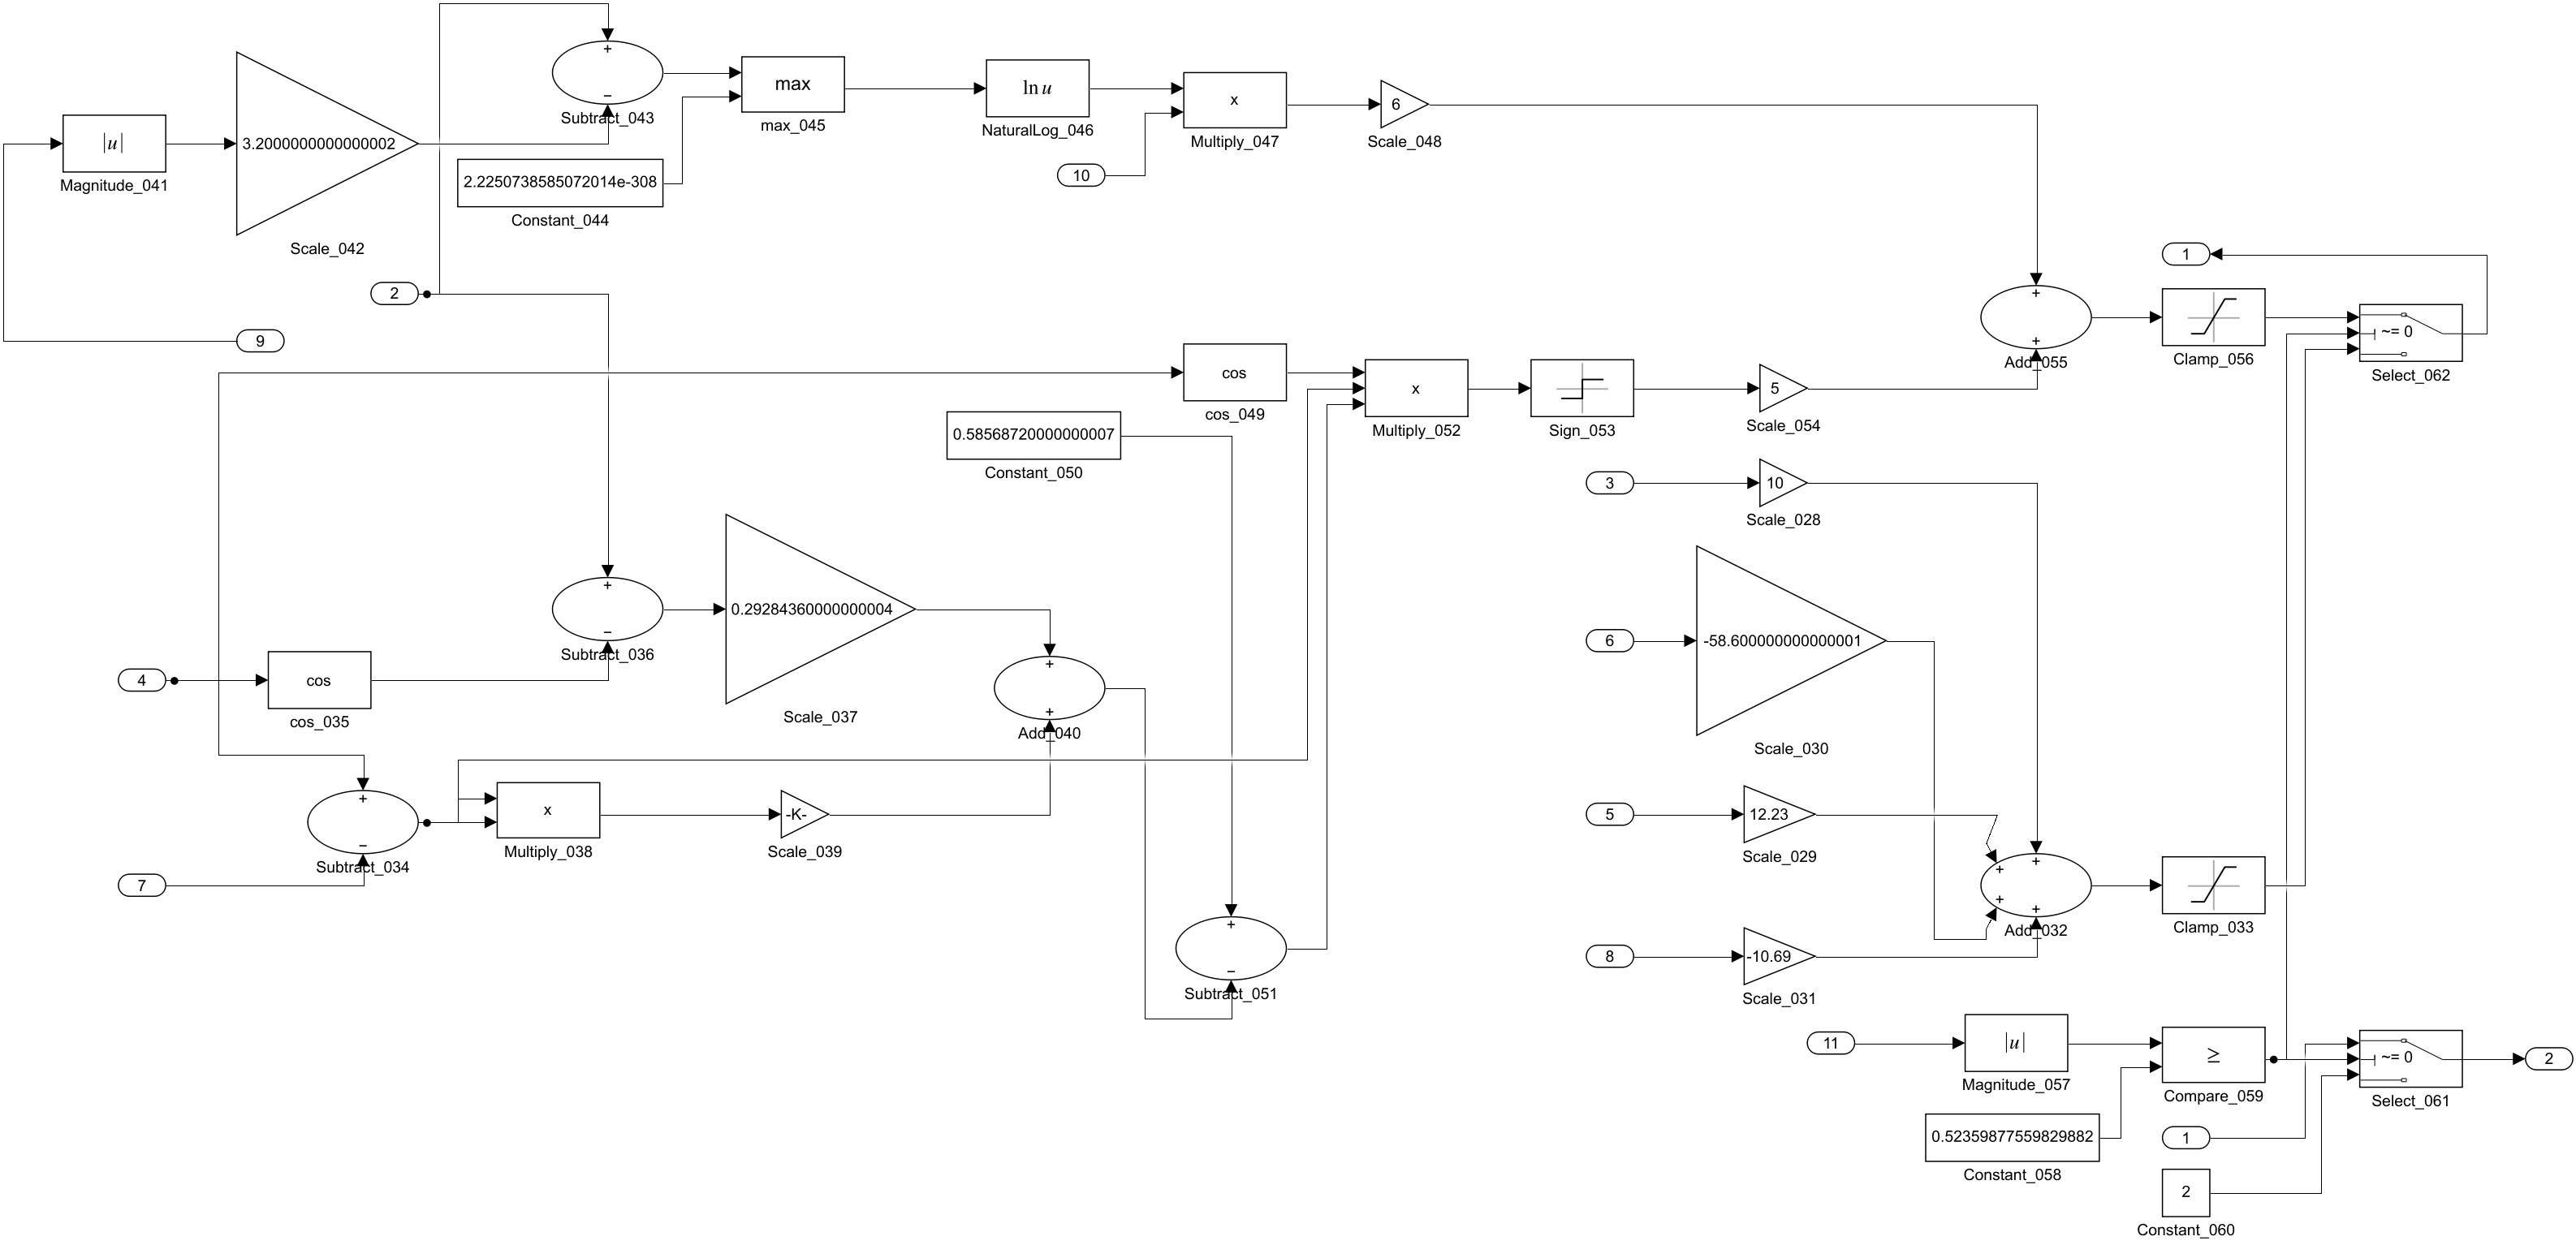
\includegraphics[width=0.85\textwidth]{docs/simulink_algorithm_guide_assets/order1_swingup_and_lqr.png}
    \caption{一级摆：摆起与 LQR 模块}
    \label{fig:o1_swingup}
\end{figure}

该模块包含两个控制分支：

\begin{itemize}
    \item 摆角离直立较远时使用\textbf{能量摆起}；
    \item 摆角进入直立邻域后使用\textbf{四状态 LQR}。
\end{itemize}

当前 LQR 控制律为：
\[
    u = 10\,x - 58.6\,\theta_1 + 12.23\,\dot{x} - 10.69\,\dot{\theta}_1
\]
加速度指令被限制在 $[-10,10]\,\text{m/s}^2$。一级阶段编号：Stage 1 能量摆起，Stage 2 LQR 稳定。算法用户可以替换能量控制、LQR、PID 或切换条件，但应继续输出\textbf{经过限幅的加速度指令}。

\subsubsection{\texorpdfstring{\texttt{Hardware/Acceleration\_to\_voltage}}{Hardware acceleration to voltage}}

\begin{figure}[htbp]
    \centering
    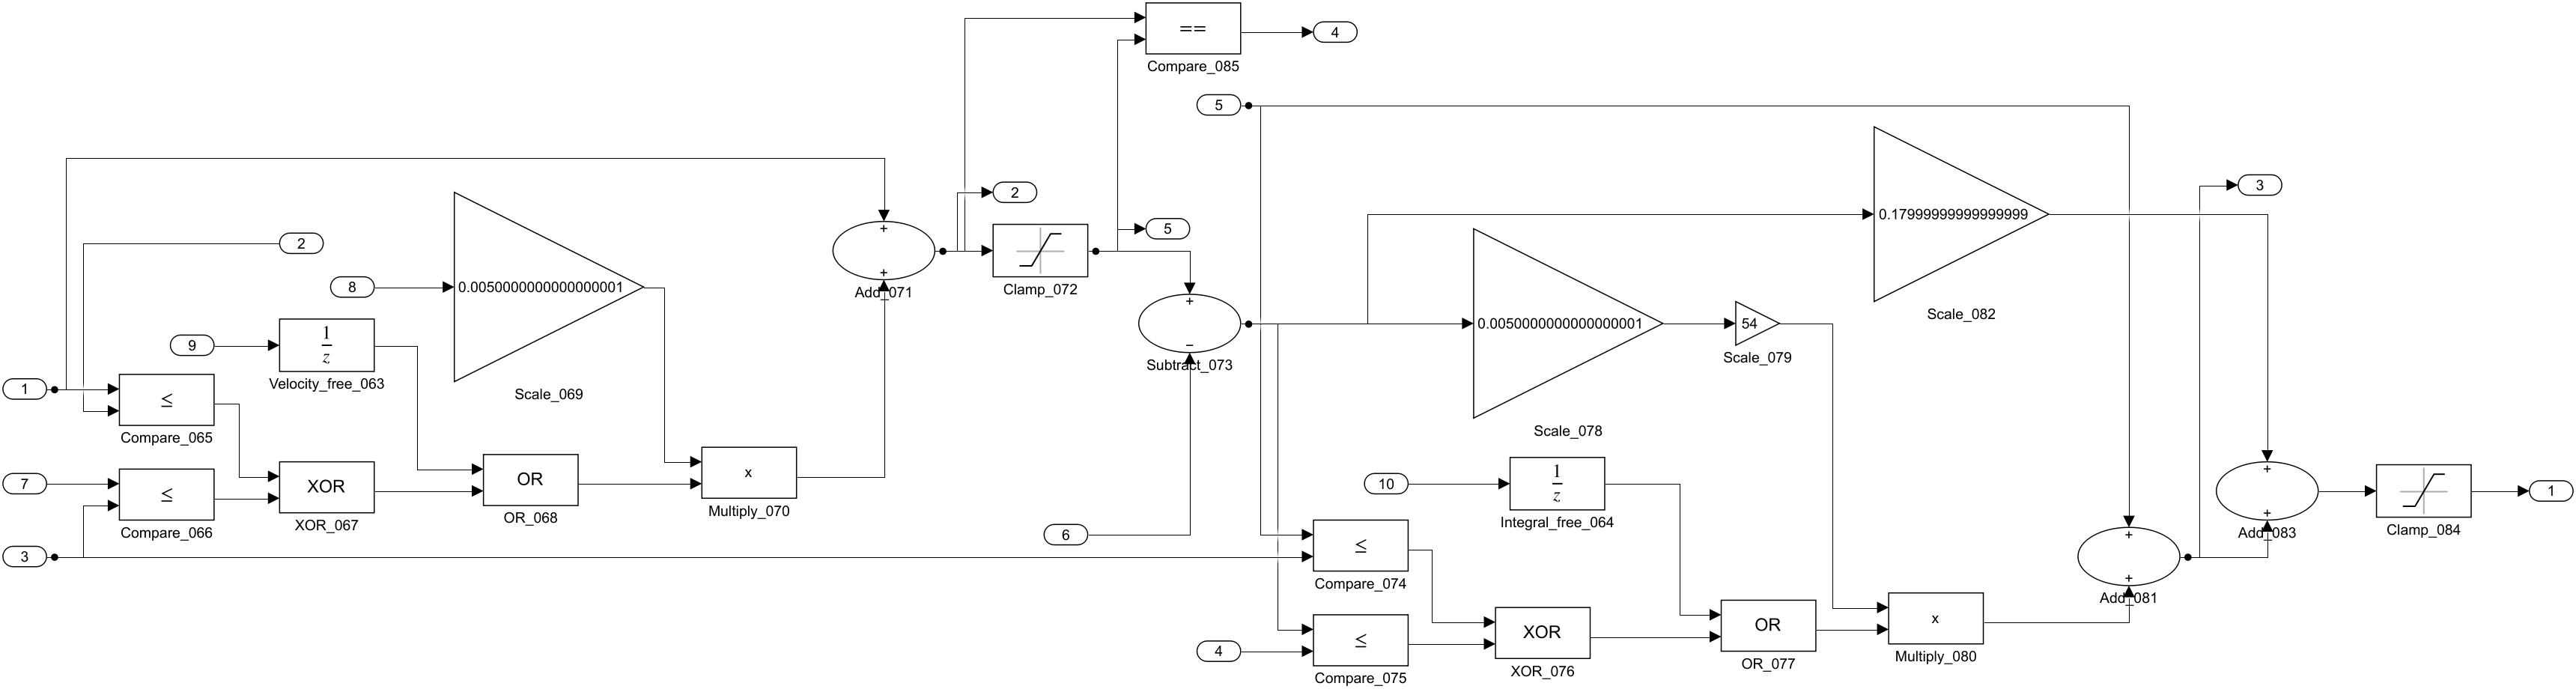
\includegraphics[width=0.9\textwidth]{docs/simulink_algorithm_guide_assets/order1_acceleration_to_voltage.png}
    \caption{一级摆：加速度到电压（执行器内环）}
    \label{fig:o1_acc2volt}
\end{figure}

这个模块不是摆杆算法本身，而是\textbf{执行器内环}：

\[
    \text{加速度指令} \;\rightarrow\; \text{离散积分得到速度参考} \;\rightarrow\; \text{与小车速度比较} \;\rightarrow\; \text{PI 速度控制}
\]
\[
    \rightarrow\; \text{电压饱和}
\]

其中包含积分器抗饱和逻辑。该模块位于不可替换的 \texttt{Hardware} 内；算法使用者只需输出加速度。

\subsubsection{\texorpdfstring{\texttt{Hardware/Travel\_and\_faults}}{Hardware travel and faults}}

\begin{figure}[htbp]
    \centering
    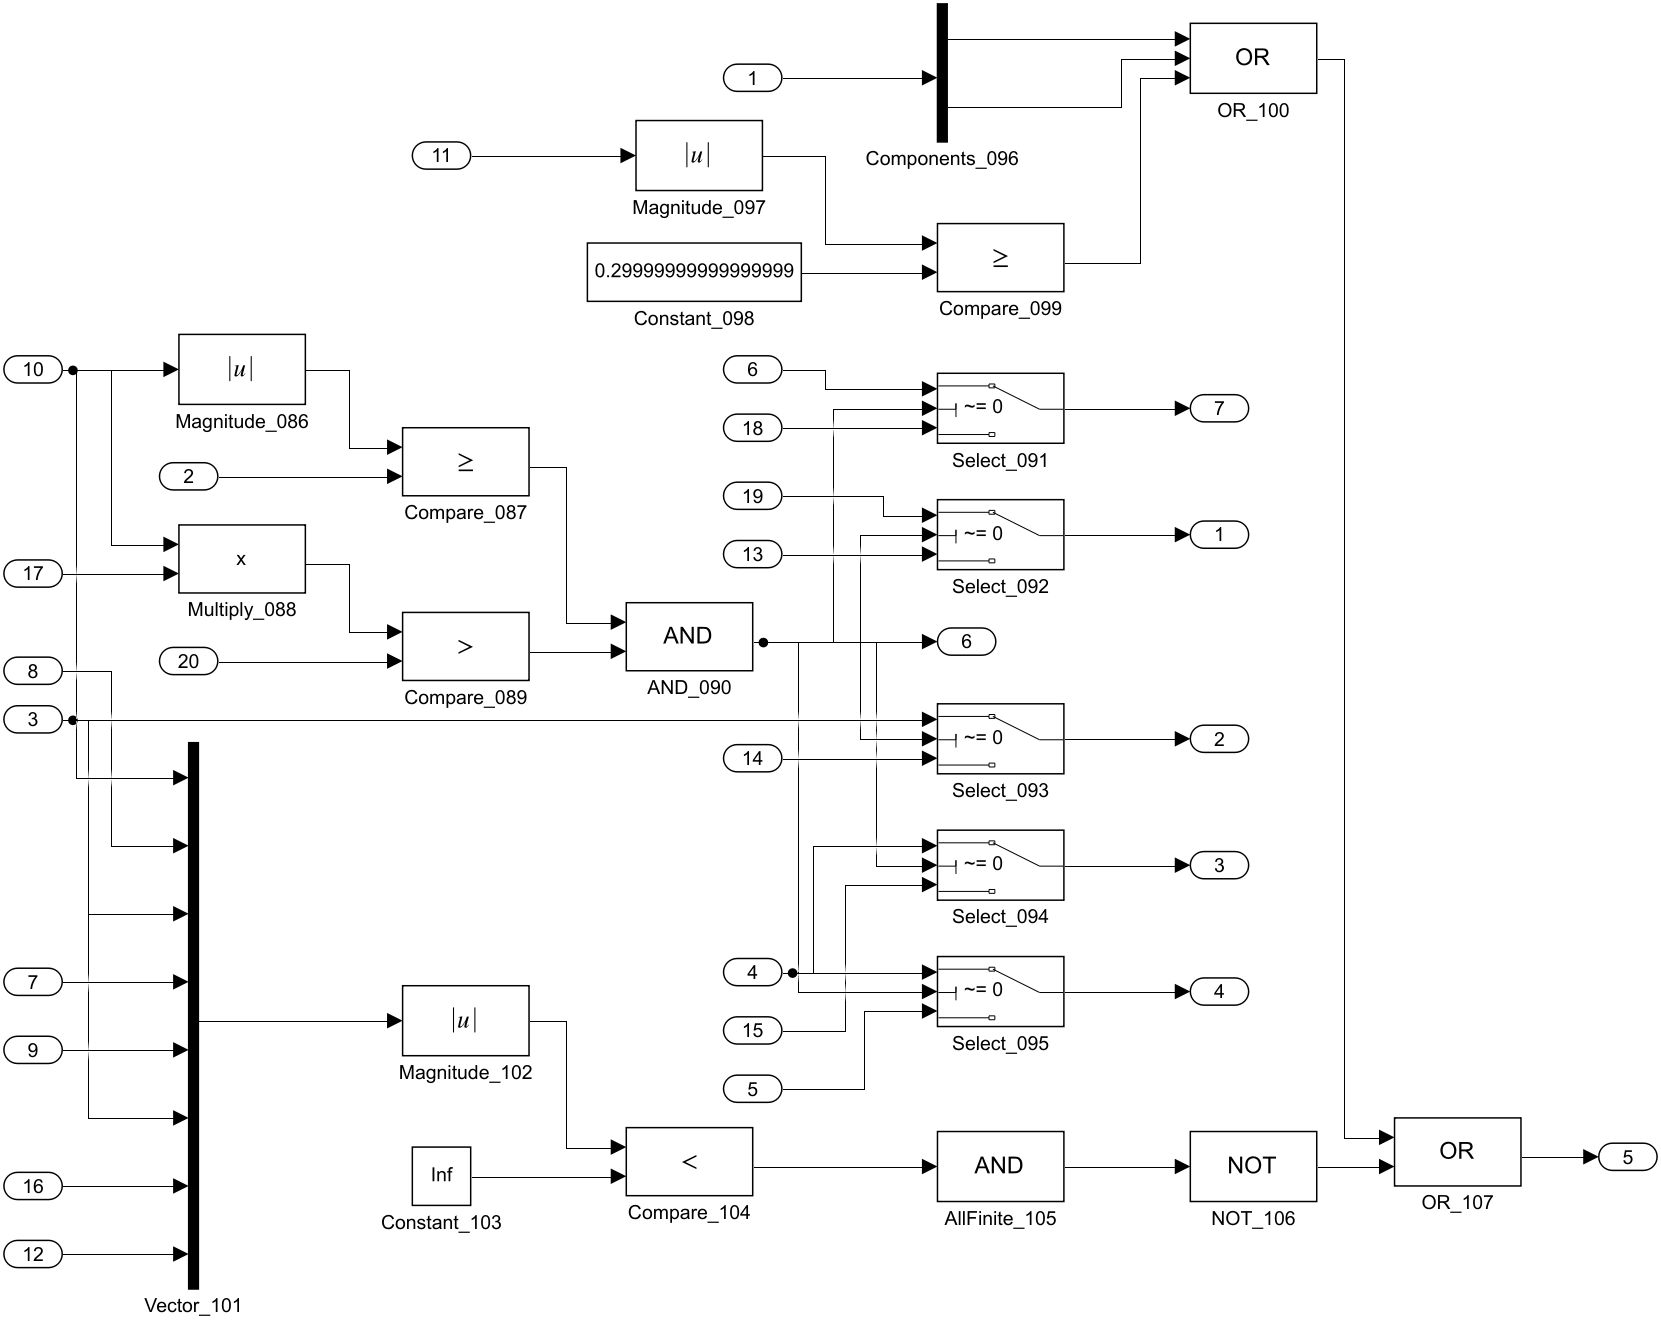
\includegraphics[width=0.65\textwidth]{docs/simulink_algorithm_guide_assets/order1_travel_and_faults.png}
    \caption{一级摆：行程与故障模块}
    \label{fig:o1_travel}
\end{figure}

该模块是\textbf{安全边界}，作用包括：

\begin{itemize}
    \item 小车达到预警位置且电压仍指向轨道外侧时，将输出置零；
    \item 清除相关积分器，避免解除限制后突然输出大电压；
    \item 检查左右物理限位、软件停止位置；
    \item 检查状态和控制结果是否为有限数值；
    \item 故障时强制 \texttt{Voltage\_V}=0 并输出 \texttt{Fault}=1。
\end{itemize}

\begin{warnbox}
    \texttt{Travel\_and\_faults} 位于 \texttt{Hardware} 内。替换 \texttt{Control} 时不得绕过或修改这条保护路径。
\end{warnbox}

\subsection{二级摆算法模块}

二级摆的 \texttt{Control} 在一级摆基础上增加了一个阶段管理模块。

\subsubsection{\texorpdfstring{\texttt{Sensor\_and\_memory}}{Sensor and memory}}

\begin{figure}[htbp]
    \centering
    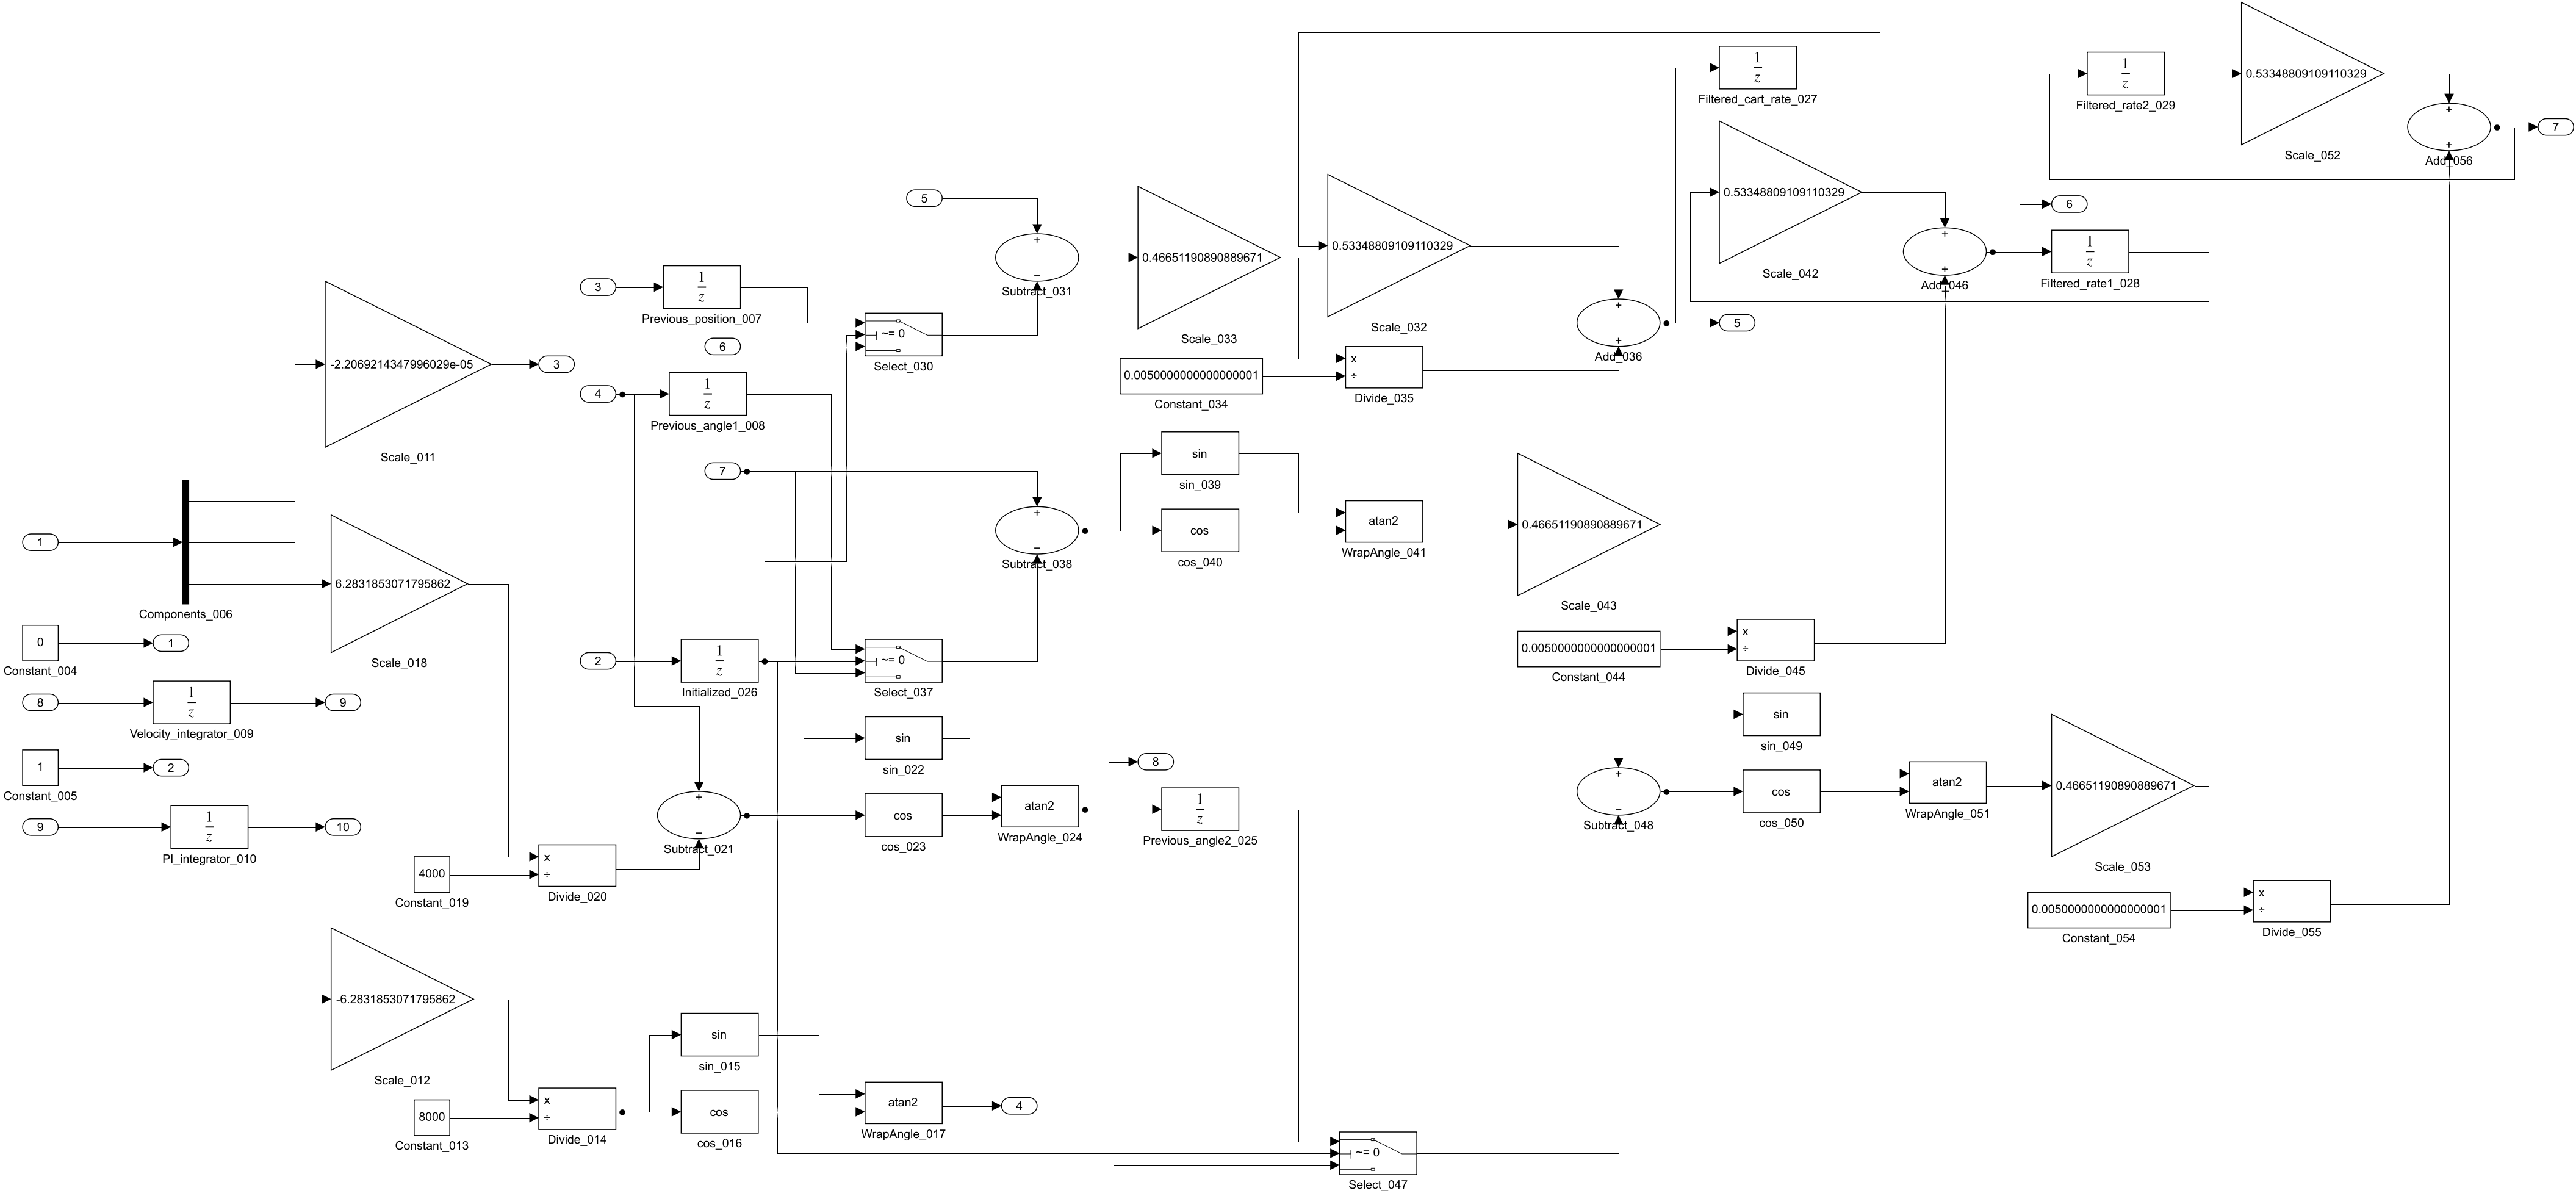
\includegraphics[width=0.7\textwidth]{docs/simulink_algorithm_guide_assets/order2_sensor_and_memory.png}
    \caption{二级摆：传感器与状态记忆模块}
    \label{fig:o2_sensor}
\end{figure}

二级模型在一级基础上增加：

\begin{itemize}
    \item 三个速度信号的一阶低通滤波；
    \item 第二摆角和角速度的上一周期状态。
\end{itemize}

控制状态顺序固定为：
\[
    [x,\ \theta_1,\ \theta_2,\ \dot{x},\ \dot{\theta}_1,\ \dot{\theta}_2]
\]
两个输入角度均以竖直向上为 0，接口单位为度；\texttt{Control} 内部转换为弧度。第二杆的相对编码器到绝对角换算已经在 \texttt{Hardware} 中完成。

\subsubsection{\texorpdfstring{\texttt{Stage\_supervisor}}{Stage supervisor}}

\begin{figure}[htbp]
    \centering
    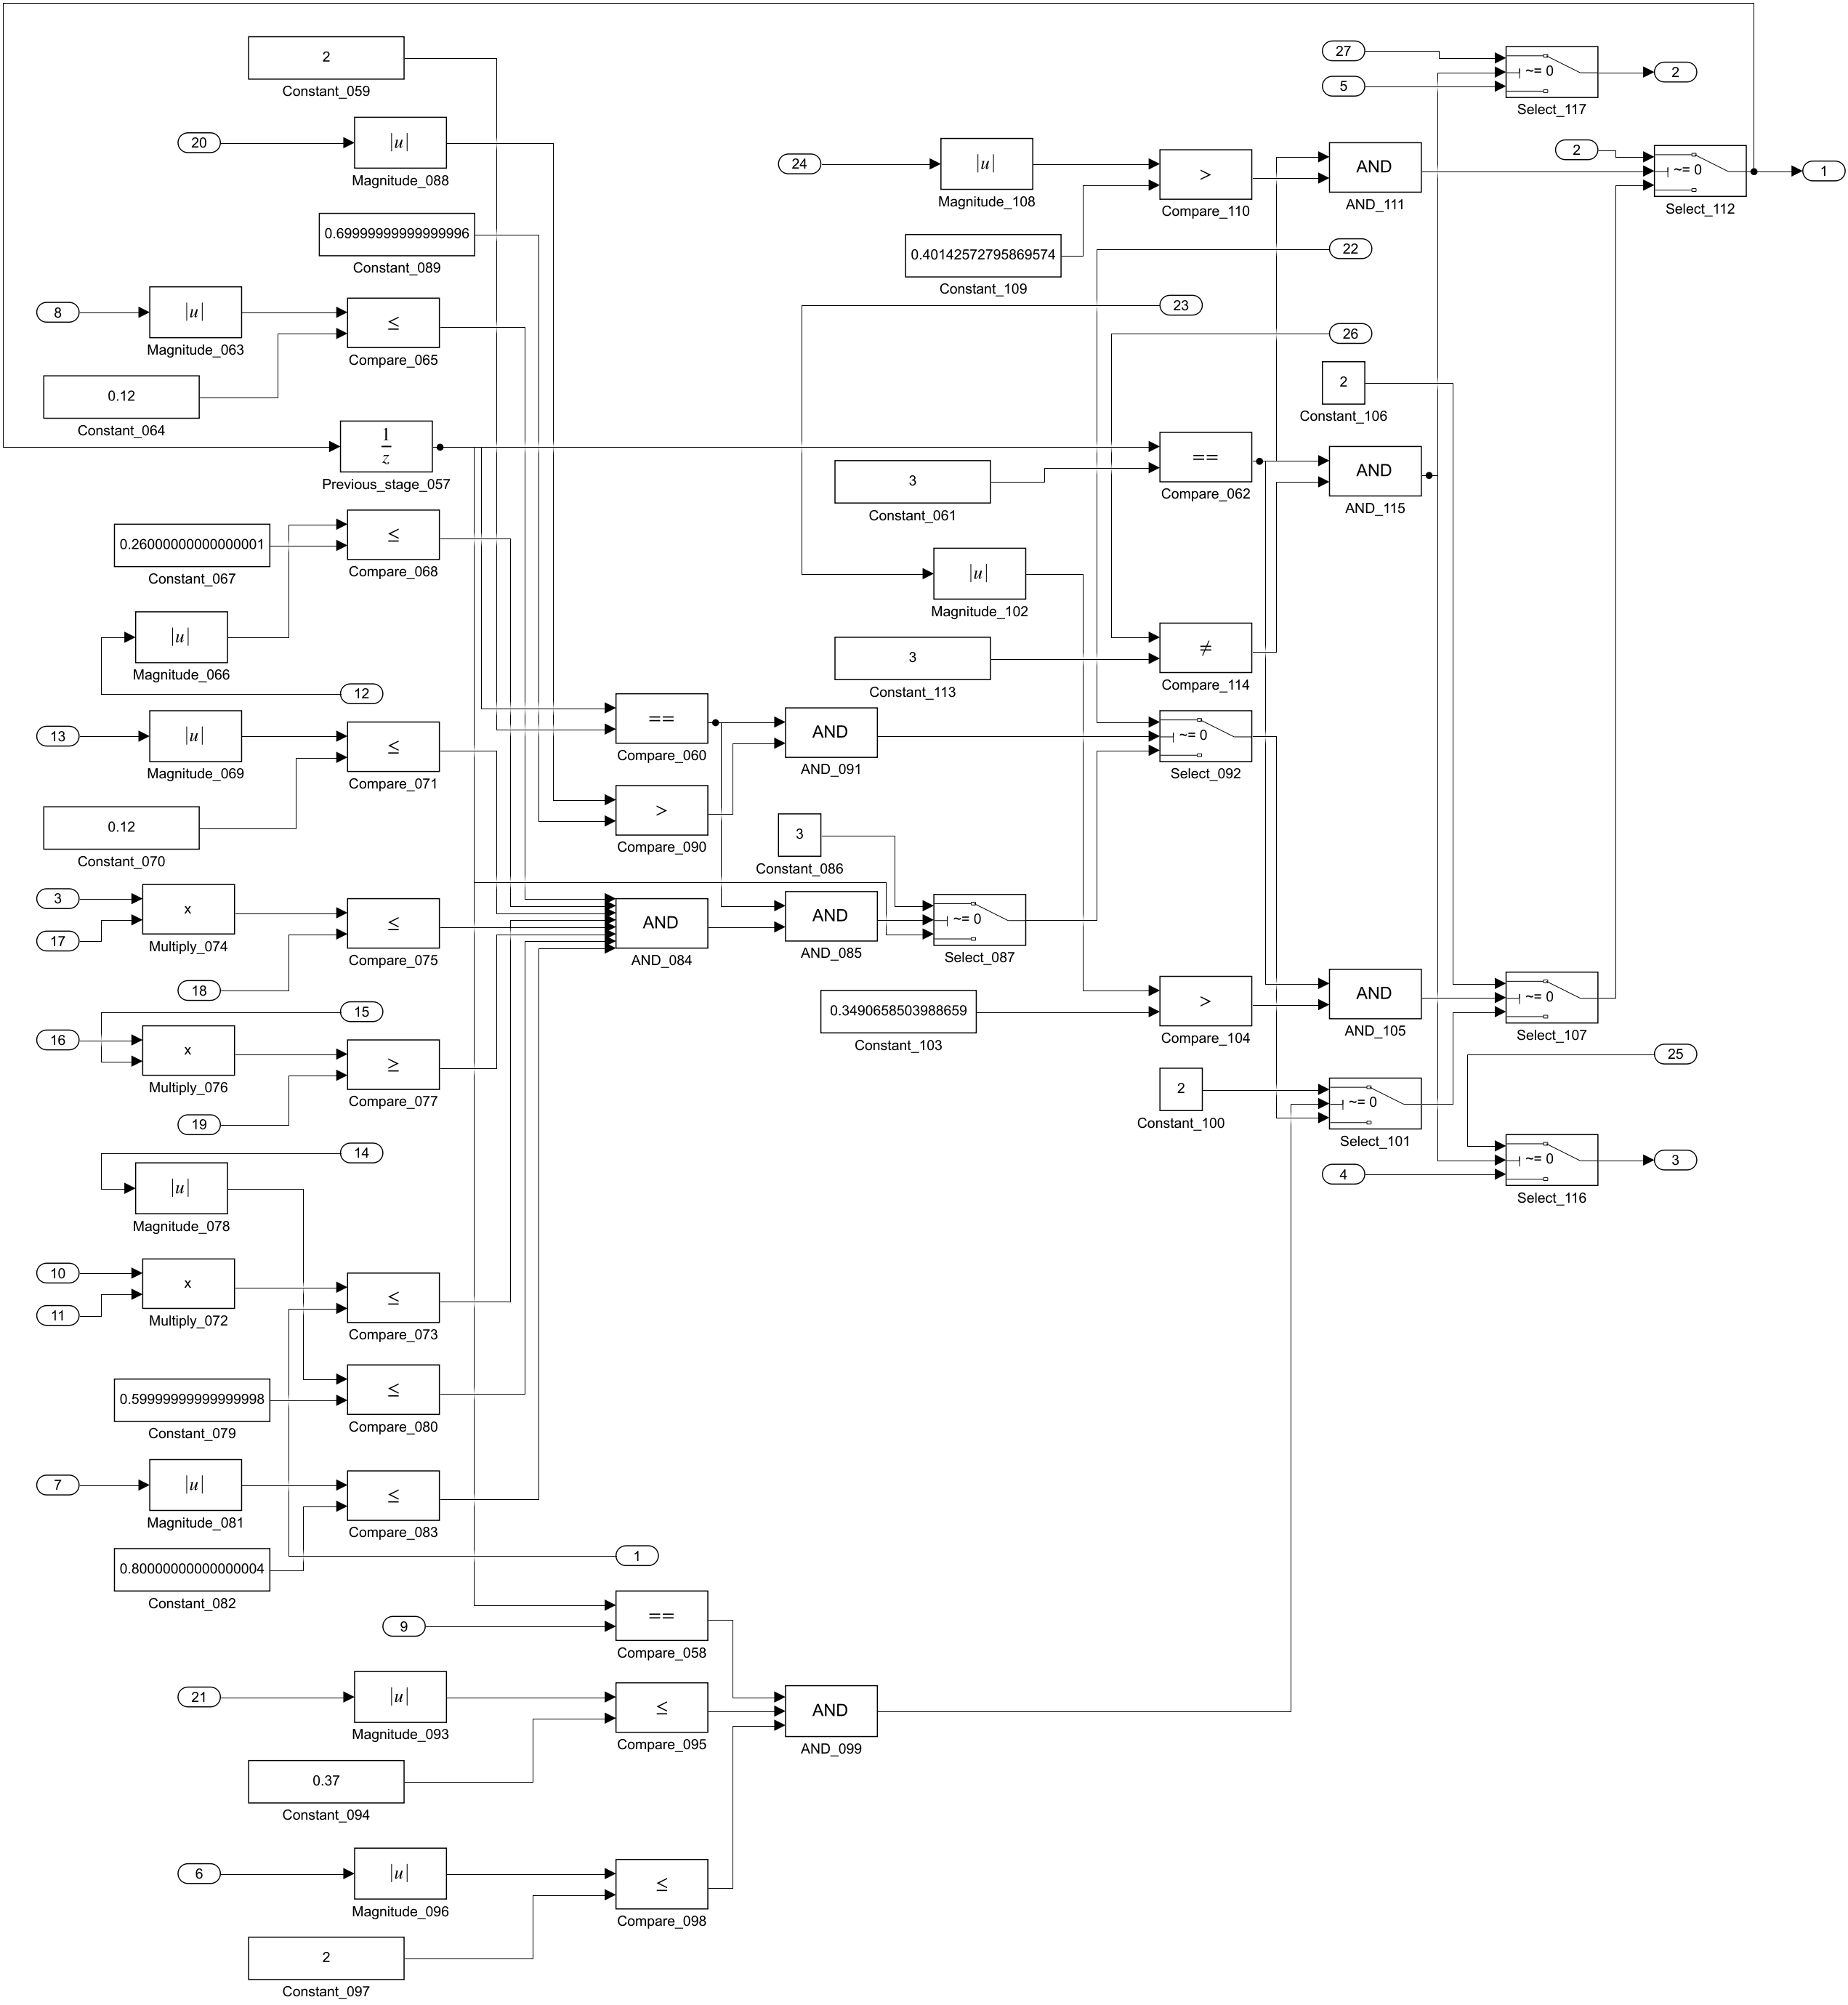
\includegraphics[width=0.55\textwidth]{docs/simulink_algorithm_guide_assets/order2_stage_supervisor.png}
    \caption{二级摆：阶段管理模块}
    \label{fig:o2_supervisor}
\end{figure}

该模块决定当前使用哪一种控制策略（阶段含义见表~\ref{tab:stages2}），根据两根摆杆的角度、角速度、小车速度和运动方向进行切换，并包含从 Stage 3 跌落后的重新进入逻辑。新版单加速度接口不向硬件层传递阶段复位信号。

\begin{tipbox}
    如果只研究直立附近控制，可以保持 Stage 3 并替换双摆稳定控制；如果研究完整摆起，则需要同时验证三个阶段及其切换条件。
\end{tipbox}

\subsubsection{\texorpdfstring{\texttt{Swingup\_and\_LQR}}{Swingup and LQR}}

\begin{figure}[htbp]
    \centering
    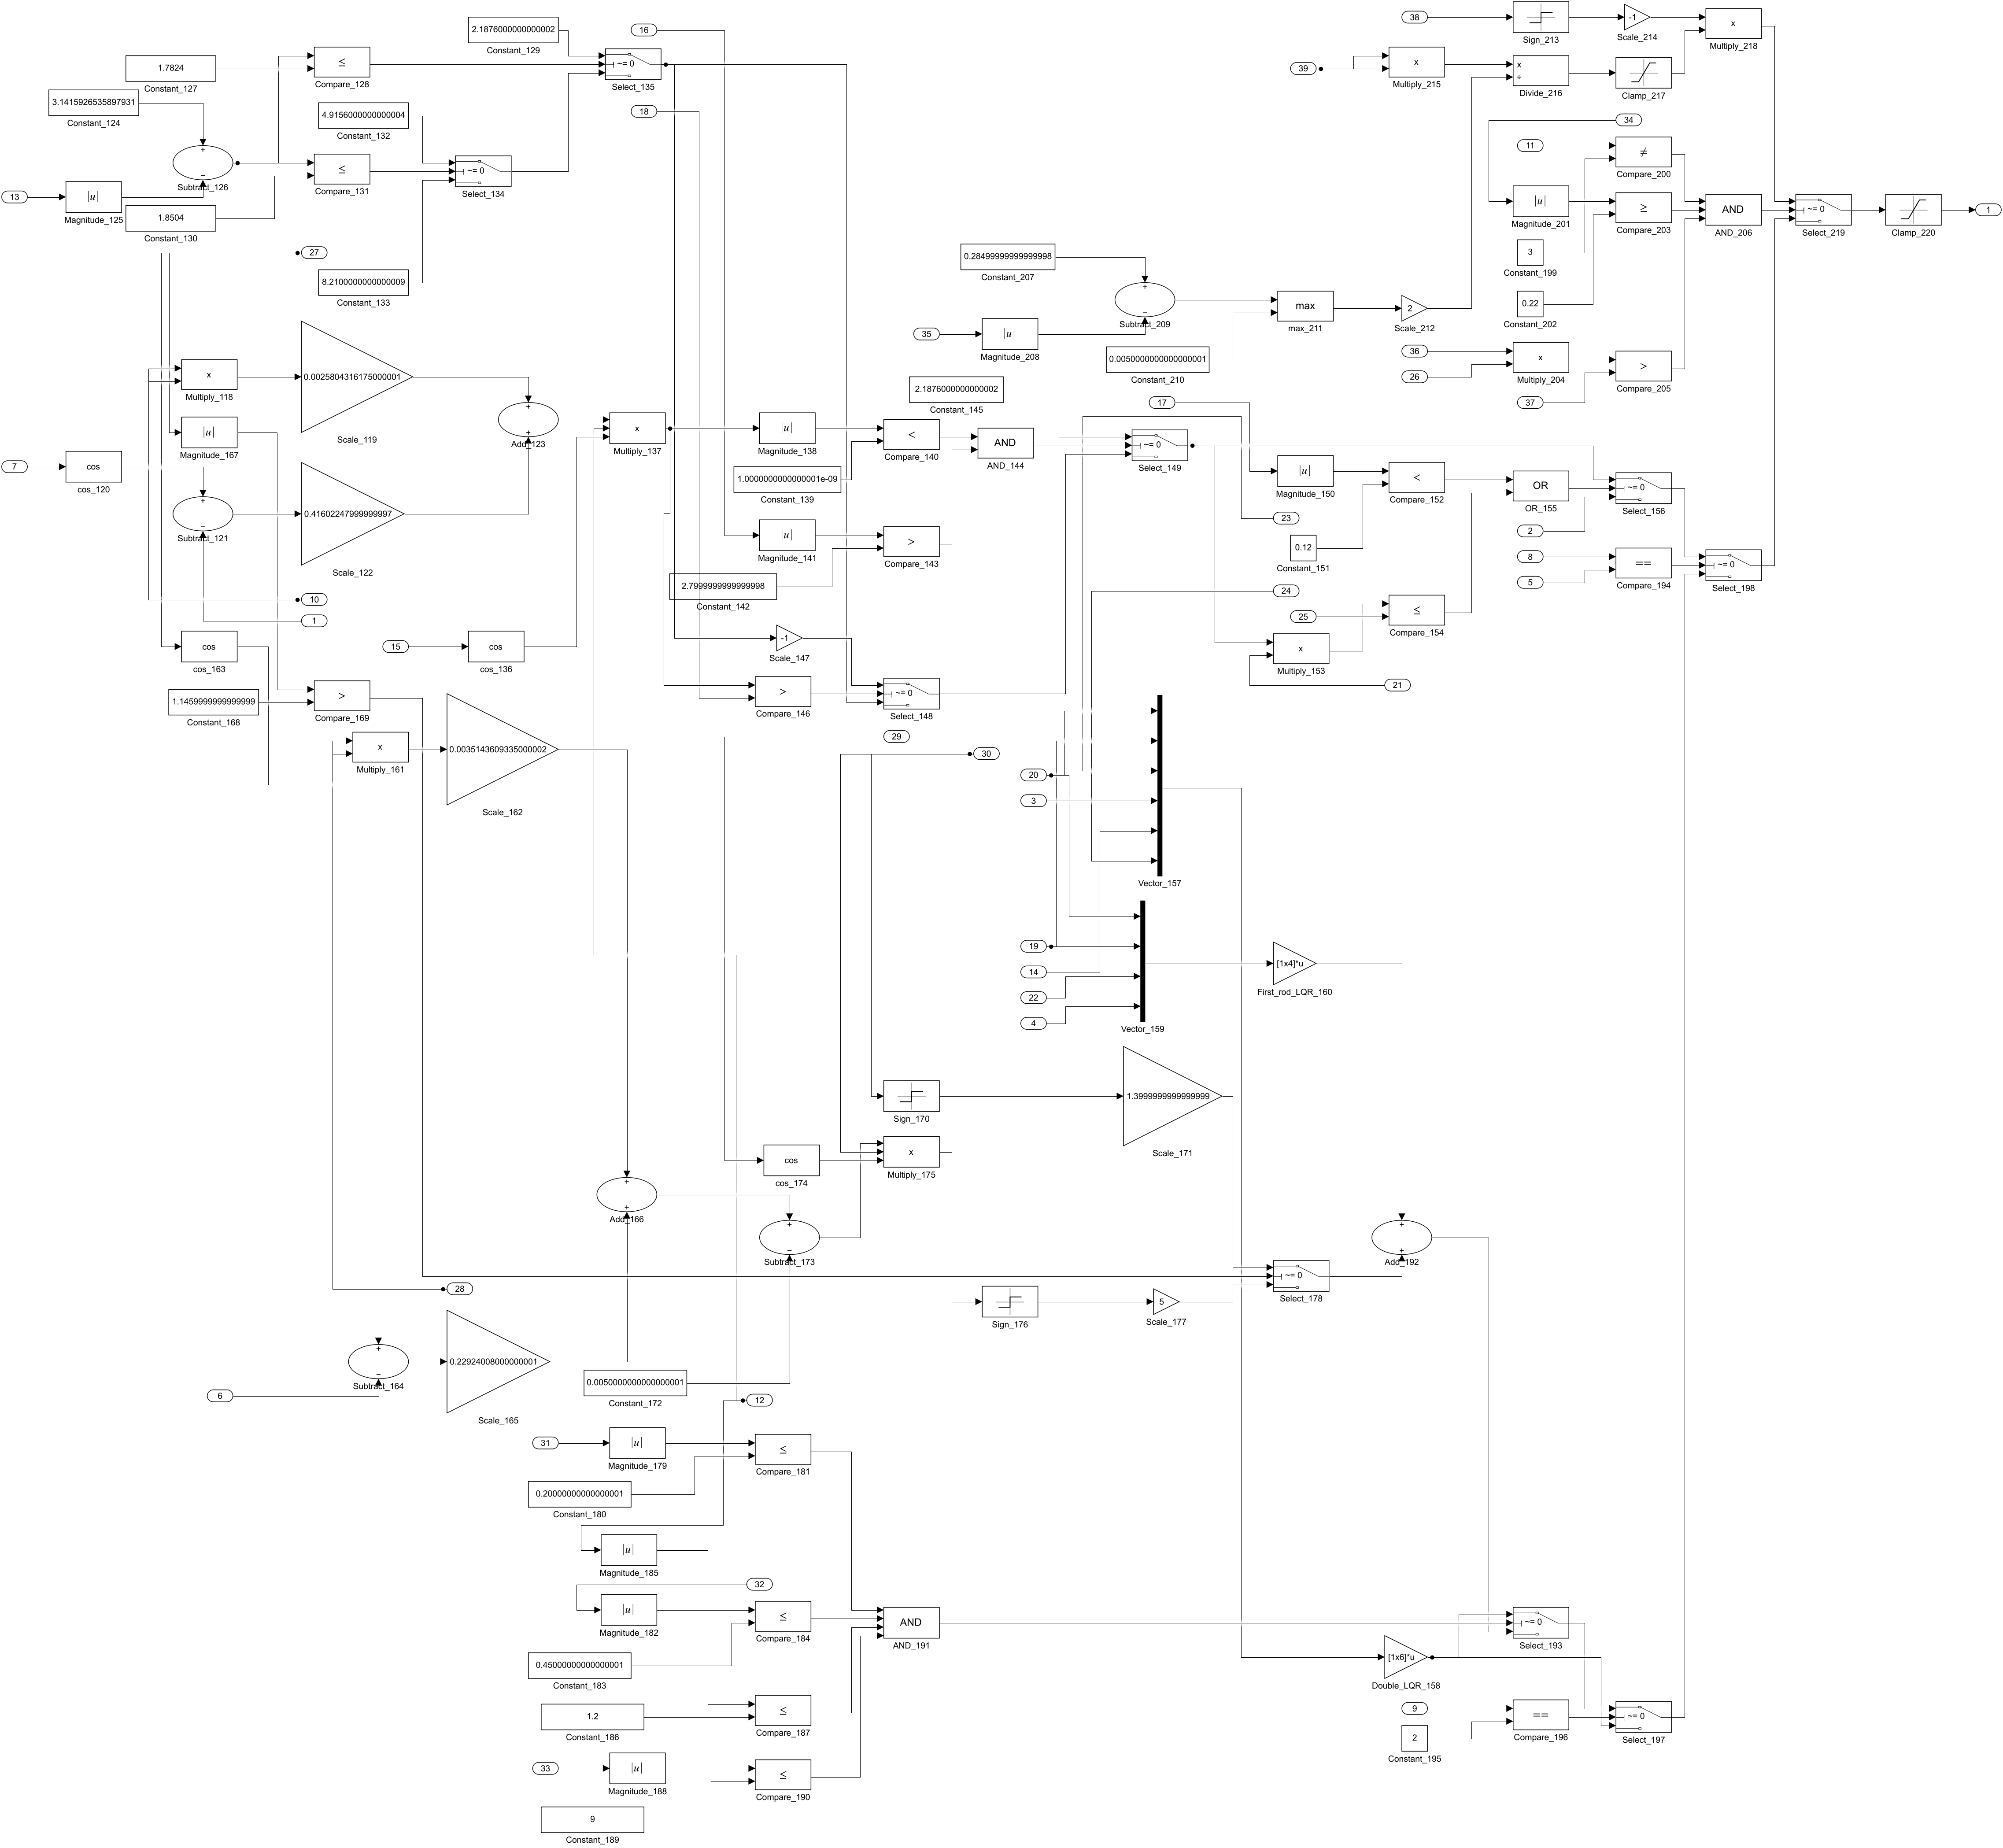
\includegraphics[width=0.62\textwidth]{docs/simulink_algorithm_guide_assets/order2_swingup_and_lqr.png}
    \caption{二级摆：摆起与 LQR 模块}
    \label{fig:o2_swingup}
\end{figure}

模块根据 \texttt{stage} 选择控制策略：

\begin{itemize}
    \item \textbf{Stage 1}：一级摆能量控制，并限制小车速度；
    \item \textbf{Stage 2}：一级摆四状态 LQR，加上第二摆能量泵入；进入捕获窗口后提前使用双摆 LQR；
    \item \textbf{Stage 3}：六状态 LQR。
\end{itemize}

六状态反馈形式为 $u = -K\,[x,\ \theta_1,\ \theta_2,\ \dot{x},\ \dot{\theta}_1,\ \dot{\theta}_2]^{\mathsf T}$，当前增益见表~\ref{tab:K2}。最终加速度限制为 $[-30,30]\,\text{m/s}^2$。接近轨道边缘并继续向外运动时，制动逻辑会覆盖普通控制指令。

\subsubsection{\texorpdfstring{\texttt{Hardware/Acceleration\_to\_voltage}}{Hardware acceleration to voltage}}

\begin{figure}[htbp]
    \centering
    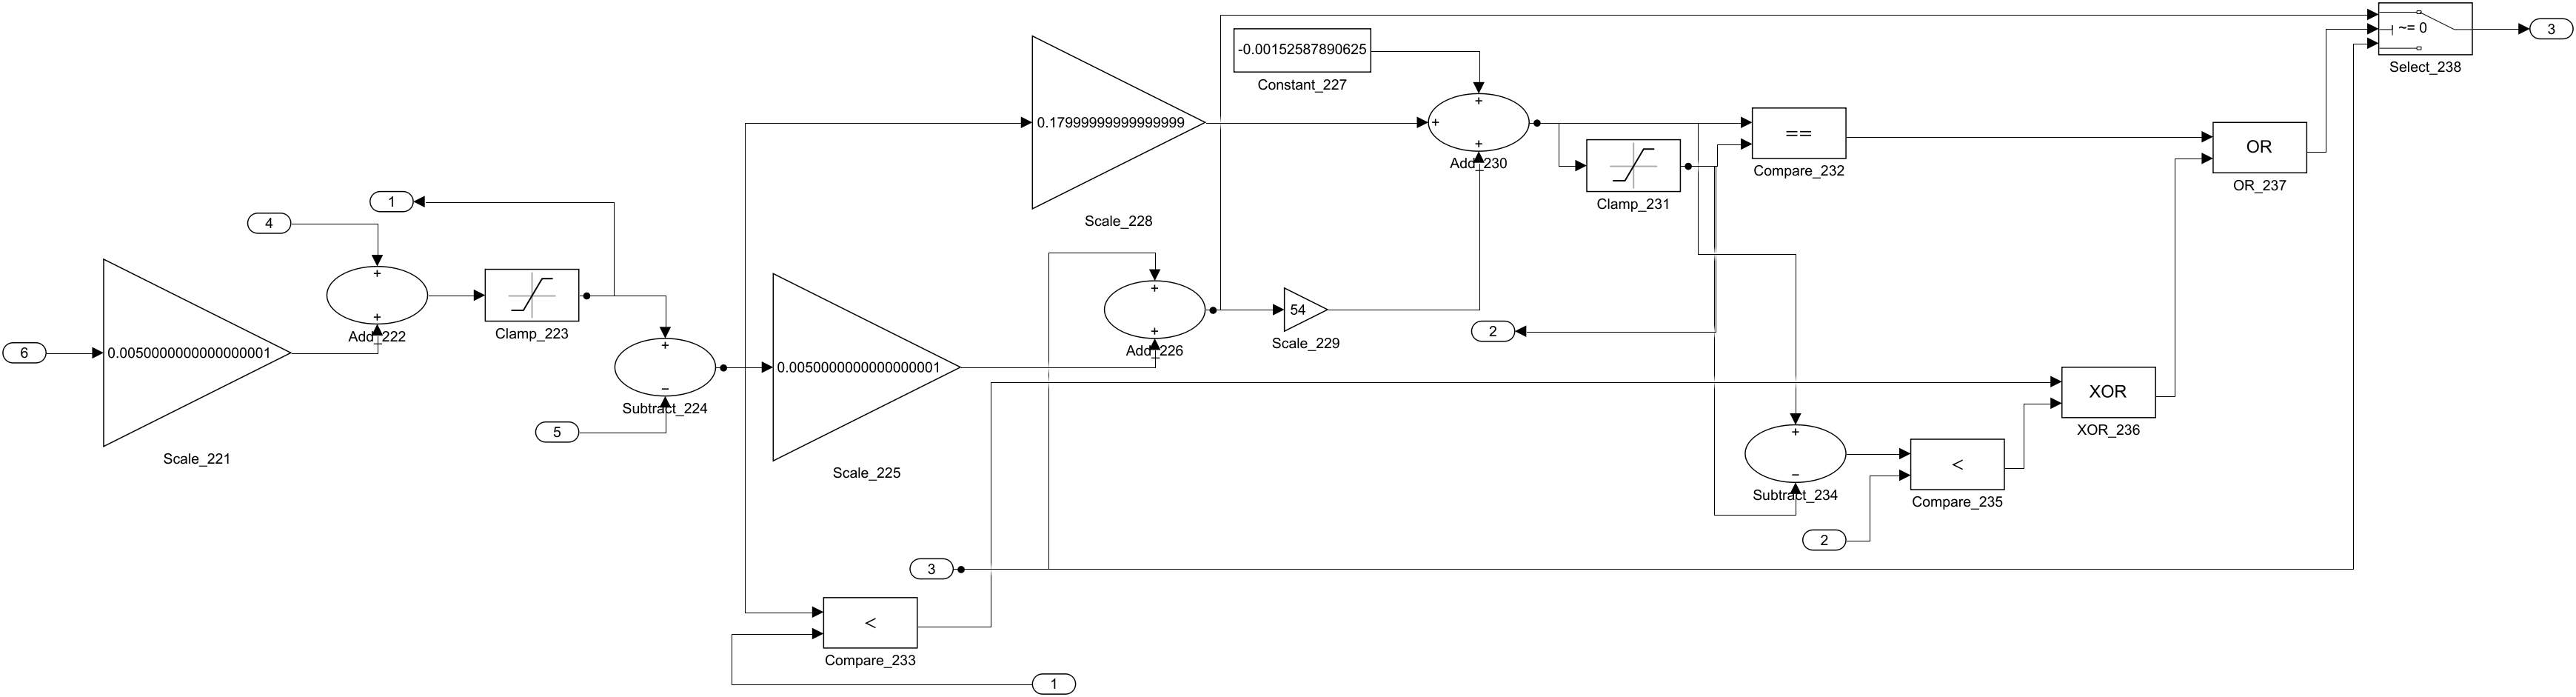
\includegraphics[width=0.85\textwidth]{docs/simulink_algorithm_guide_assets/order2_acceleration_to_voltage.png}
    \caption{二级摆：加速度到电压（执行器内环）}
    \label{fig:o2_acc2volt}
\end{figure}

作用与一级模型相同：加速度积分为速度参考，再由 PI 速度环生成电压。当前约束为：

\begin{itemize}
    \item 速度参考：$[-0.6,0.6]\,\text{m/s}$；
    \item 电压：$[-1,1]\,\text{V}$；
    \item 包含电压饱和条件下的积分抗饱和；
    \item 加入已标定的静止补偿电压。
\end{itemize}

\subsubsection{\texorpdfstring{\texttt{Hardware/Travel\_and\_faults}}{Hardware travel and faults}}

\begin{figure}[htbp]
    \centering
    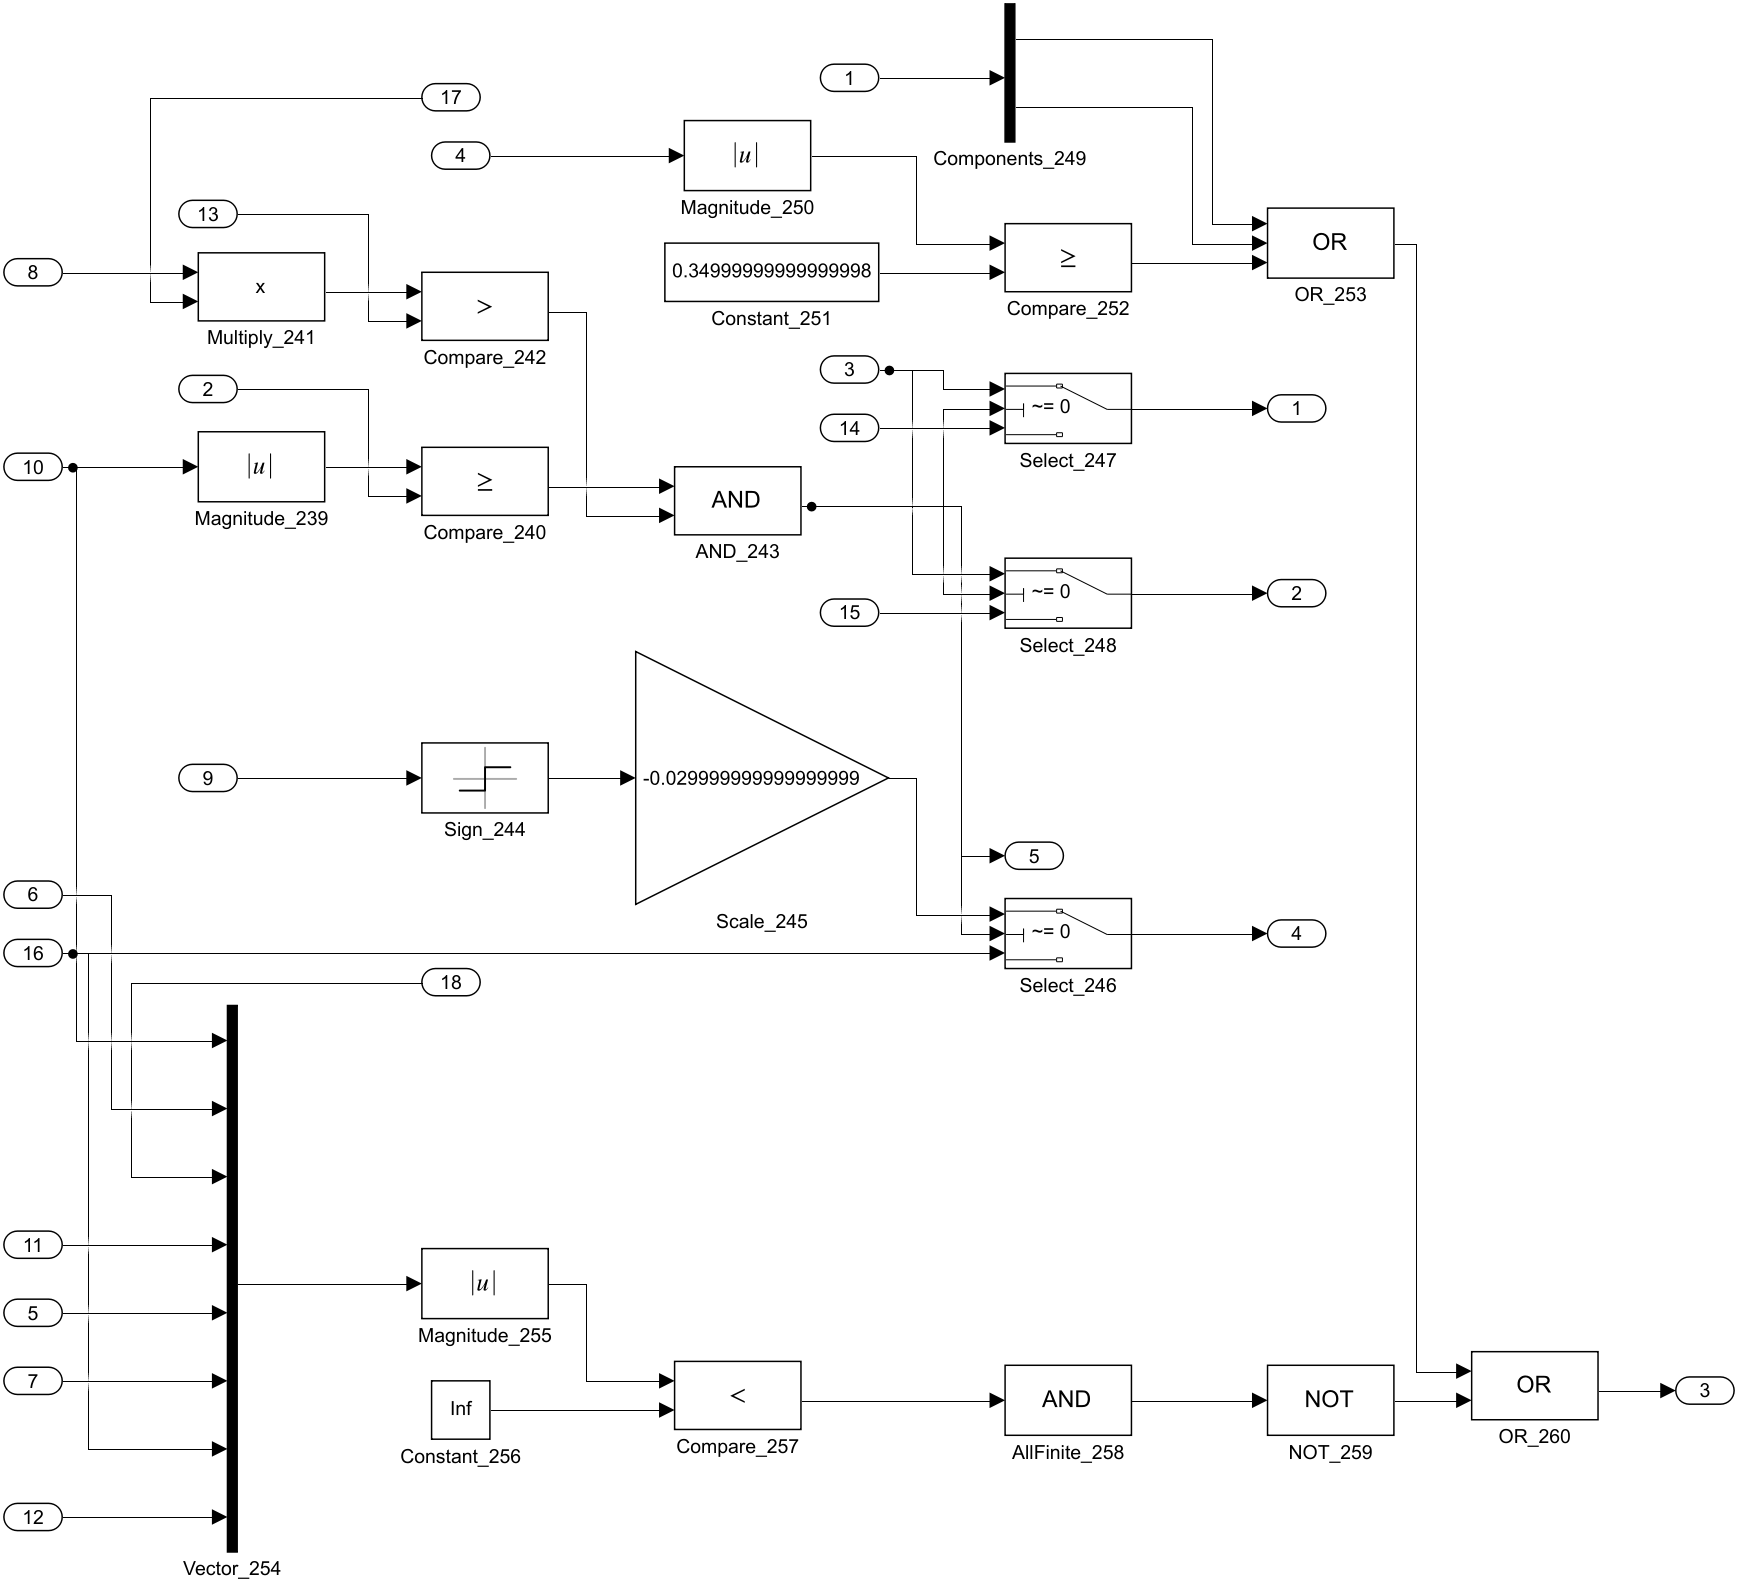
\includegraphics[width=0.6\textwidth]{docs/simulink_algorithm_guide_assets/order2_travel_and_faults.png}
    \caption{二级摆：行程与故障模块}
    \label{fig:o2_travel}
\end{figure}

与一级模型的不同之处：达到预警位置且控制仍指向外侧时，不是简单输出 0\,V，而是施加 $0.03\,\text{V}$ 的\textbf{向中心恢复电压}，同时清除控制积分状态。物理限位、软件停止位置或非有限数值仍会立即产生故障并输出 0\,V。

% ======================================================================
\section{MATLAB 离线仿真}
\label{sec:matlab}

\subsection{离线仿真能做什么}

离线仿真的模型不连接真实板卡，适合在修改实机 \texttt{Control} 前验证算法。典型用途包括：参数搜索、批量测试、LQR 增益设计与优化、验证摆起/稳摆的收敛性。

\begin{warnbox}
    离线仿真中效果良好\textbf{不代表可以直接安全运行实机}。迁移前还要检查采样周期、编码器方向、输出单位、执行器饱和和安全限制（见第~\ref{sec:migration} 节）。
\end{warnbox}

\subsection{快速运行}

在 MATLAB 中将当前目录切换到项目根目录，然后执行：

\begin{lstlisting}[language=Matlab, caption={离线仿真快速运行}, label={lst:quick}]
addpath('matlab');
setup_pendulum;

single_swing = run_pendulum('single','swingup');
single_hold  = run_pendulum('single','balance');
double_swing = run_pendulum('double','swingup');
double_hold  = run_pendulum('double','balance');
\end{lstlisting}

每次运行都会在 \texttt{matlab/output/<类型>\_pendulum/} 下创建独立目录并保存结果 MAT 文件，不会覆盖上一轮结果。

\subsection{统一入口与参数}

\begin{lstlisting}[caption={run\_pendulum 统一入口与调用关系}, label={lst:call}]
run_pendulum(order, scenario, options)
|
|-- single
|   |-- numeric   -> sp_simulate -> sp_control + sp_dynamics -> sp_metrics
|   `-- simulink  -> sp_build_model -> sim -> sp_metrics
|
`-- double
    |-- numeric swingup -> dp_simulate_swingup
    |-- numeric balance -> dp_simulate_numeric
    `-- simulink        -> run_simulation -> build_model -> sim
\end{lstlisting}

\begin{center}
    \renewcommand{\arraystretch}{1.4}
    \begin{tabular}{@{}l l p{8.4cm}@{}}
        \toprule
        \textbf{参数} & \textbf{可选值} & \textbf{含义} \\
        \midrule
        \texttt{order} & \texttt{single}, \texttt{double} & 一级摆或二级摆 \\
        \texttt{scenario} & \texttt{swingup}, \texttt{balance} & 完整摆起或直立附近稳摆 \\
        \texttt{options.engine} & \texttt{numeric}, \texttt{simulink} & 数值积分或 Simulink 引擎 \\
        \bottomrule
    \end{tabular}
\end{center}

\begin{tipbox}
    \texttt{numeric} 引擎适合参数搜索和批量测试；\texttt{simulink} 引擎适合检查模型结构、采样保持和信号连接。
\end{tipbox}

\subsection{一级摆离线模型}

\begin{figure}[htbp]
    \centering
    \begin{subfigure}{0.48\textwidth}
        \centering
        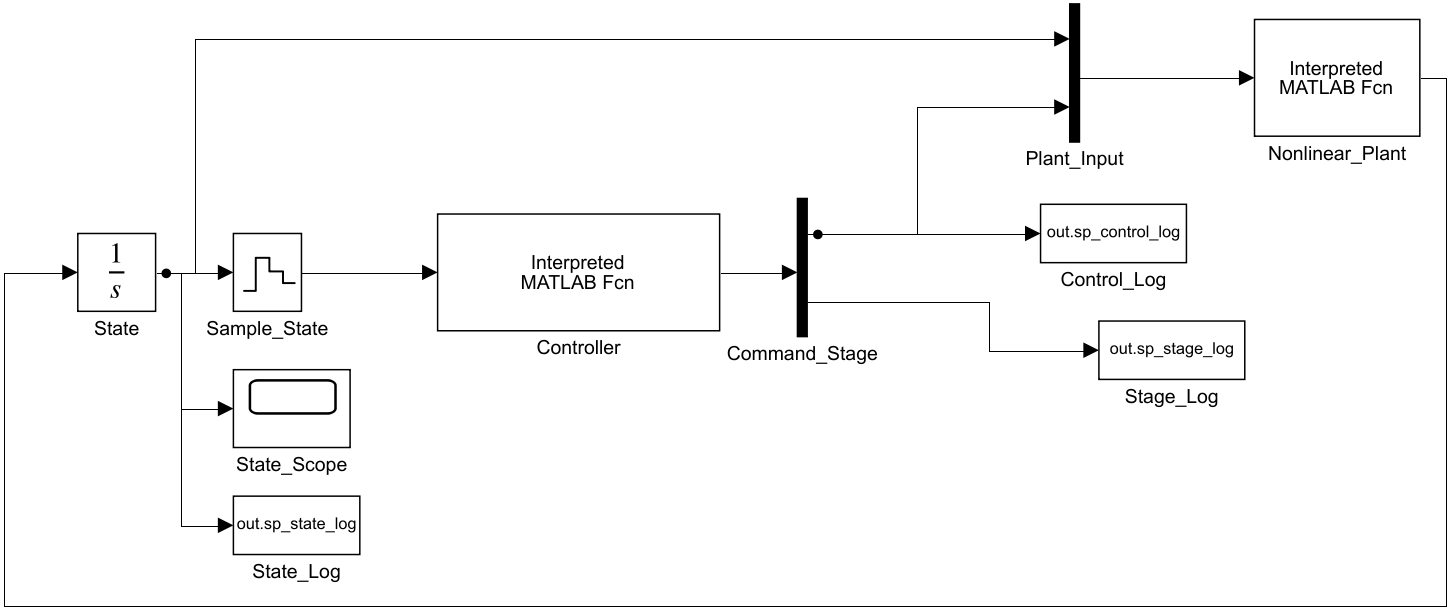
\includegraphics[width=\textwidth]{docs/matlab_simulation_lqr_assets/single_pendulum_swingup.png}
        \caption{一级摆摆起模型}
    \end{subfigure}
    \hfill
    \begin{subfigure}{0.48\textwidth}
        \centering
        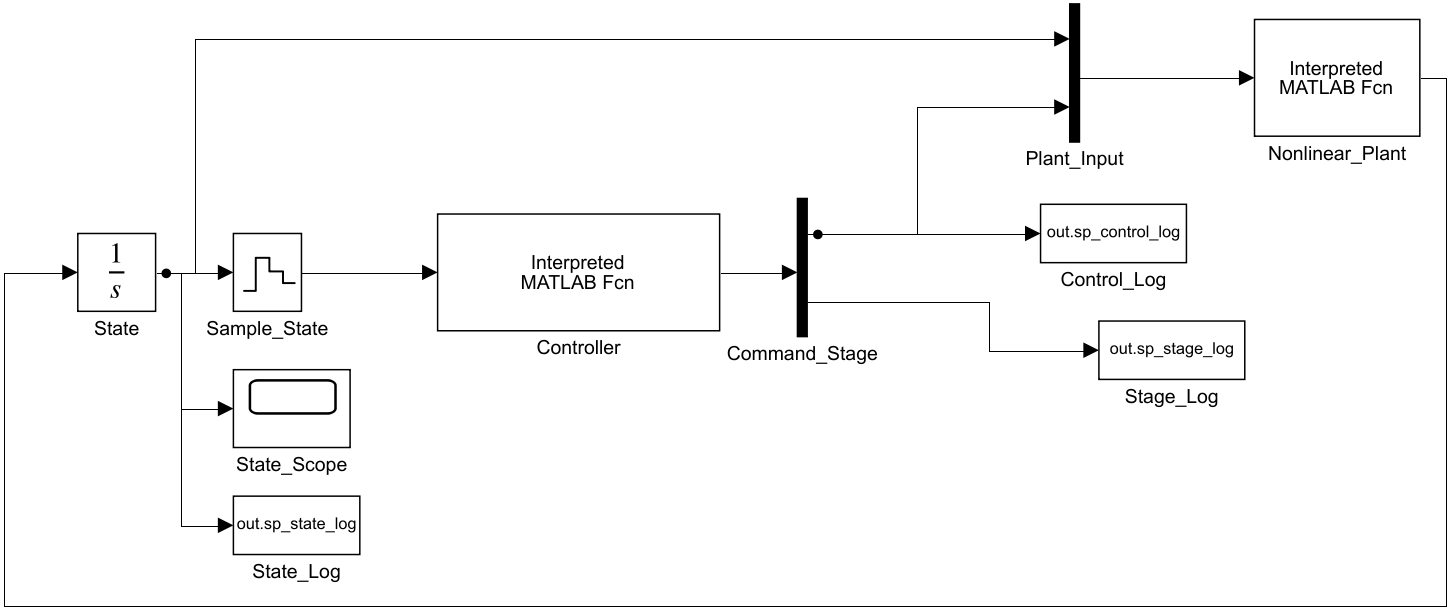
\includegraphics[width=\textwidth]{docs/matlab_simulation_lqr_assets/single_pendulum_balance.png}
        \caption{一级摆稳摆模型}
    \end{subfigure}
    \caption{一级摆离线 Simulink 模型}
    \label{fig:sp_models}
\end{figure}

两个模型结构相同，主要区别是初始状态和控制器是否允许进入摆起分支。一级状态定义：

\[
    X = [x,\ \theta,\ \dot{x},\ \dot{\theta}]^{\mathsf T}
\]

\begin{itemize}
    \item $x$：小车位置，单位 m；
    \item $\theta$：摆杆角度，直立向上为 0，单位 rad；
    \item $\dot{x}$：小车速度，单位 m/s；
    \item $\dot{\theta}$：摆杆角速度，单位 rad/s；
    \item $u$：小车加速度指令，单位 m/s$^2$。
\end{itemize}

\subsection{二级摆离线模型}

\begin{figure}[htbp]
    \centering
    \begin{subfigure}{0.48\textwidth}
        \centering
        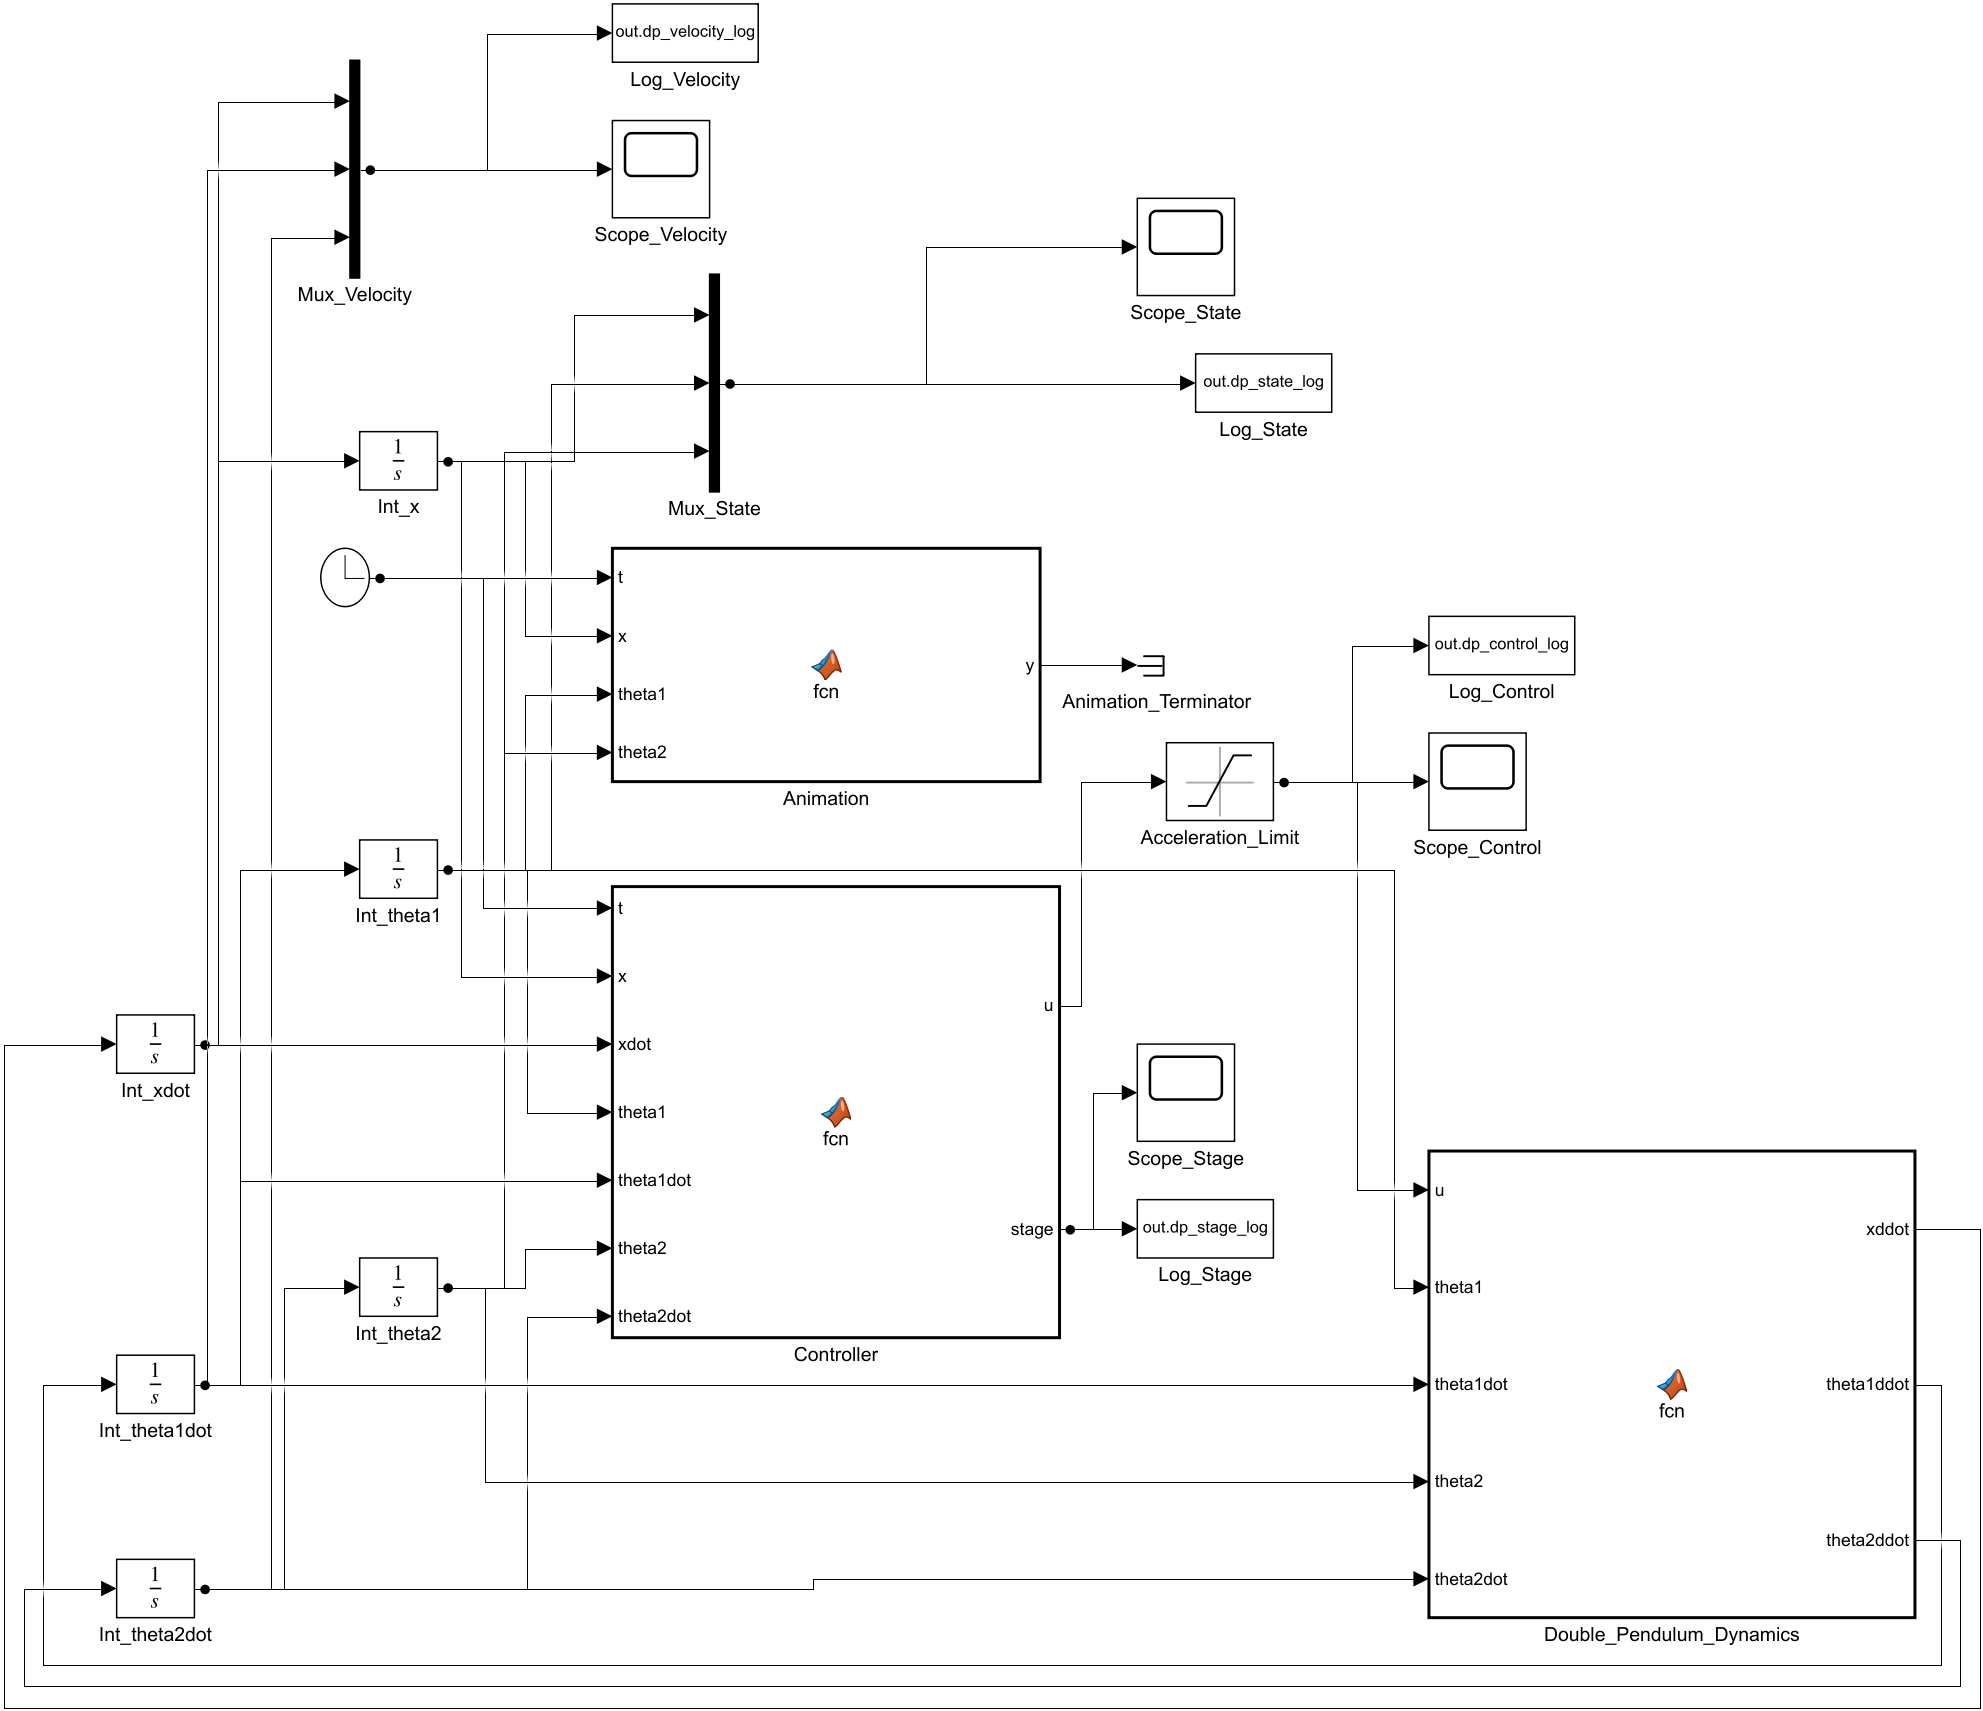
\includegraphics[width=\textwidth]{docs/matlab_simulation_lqr_assets/double_pendulum_project.png}
        \caption{二级摆完整摆起模型}
    \end{subfigure}
    \hfill
    \begin{subfigure}{0.48\textwidth}
        \centering
        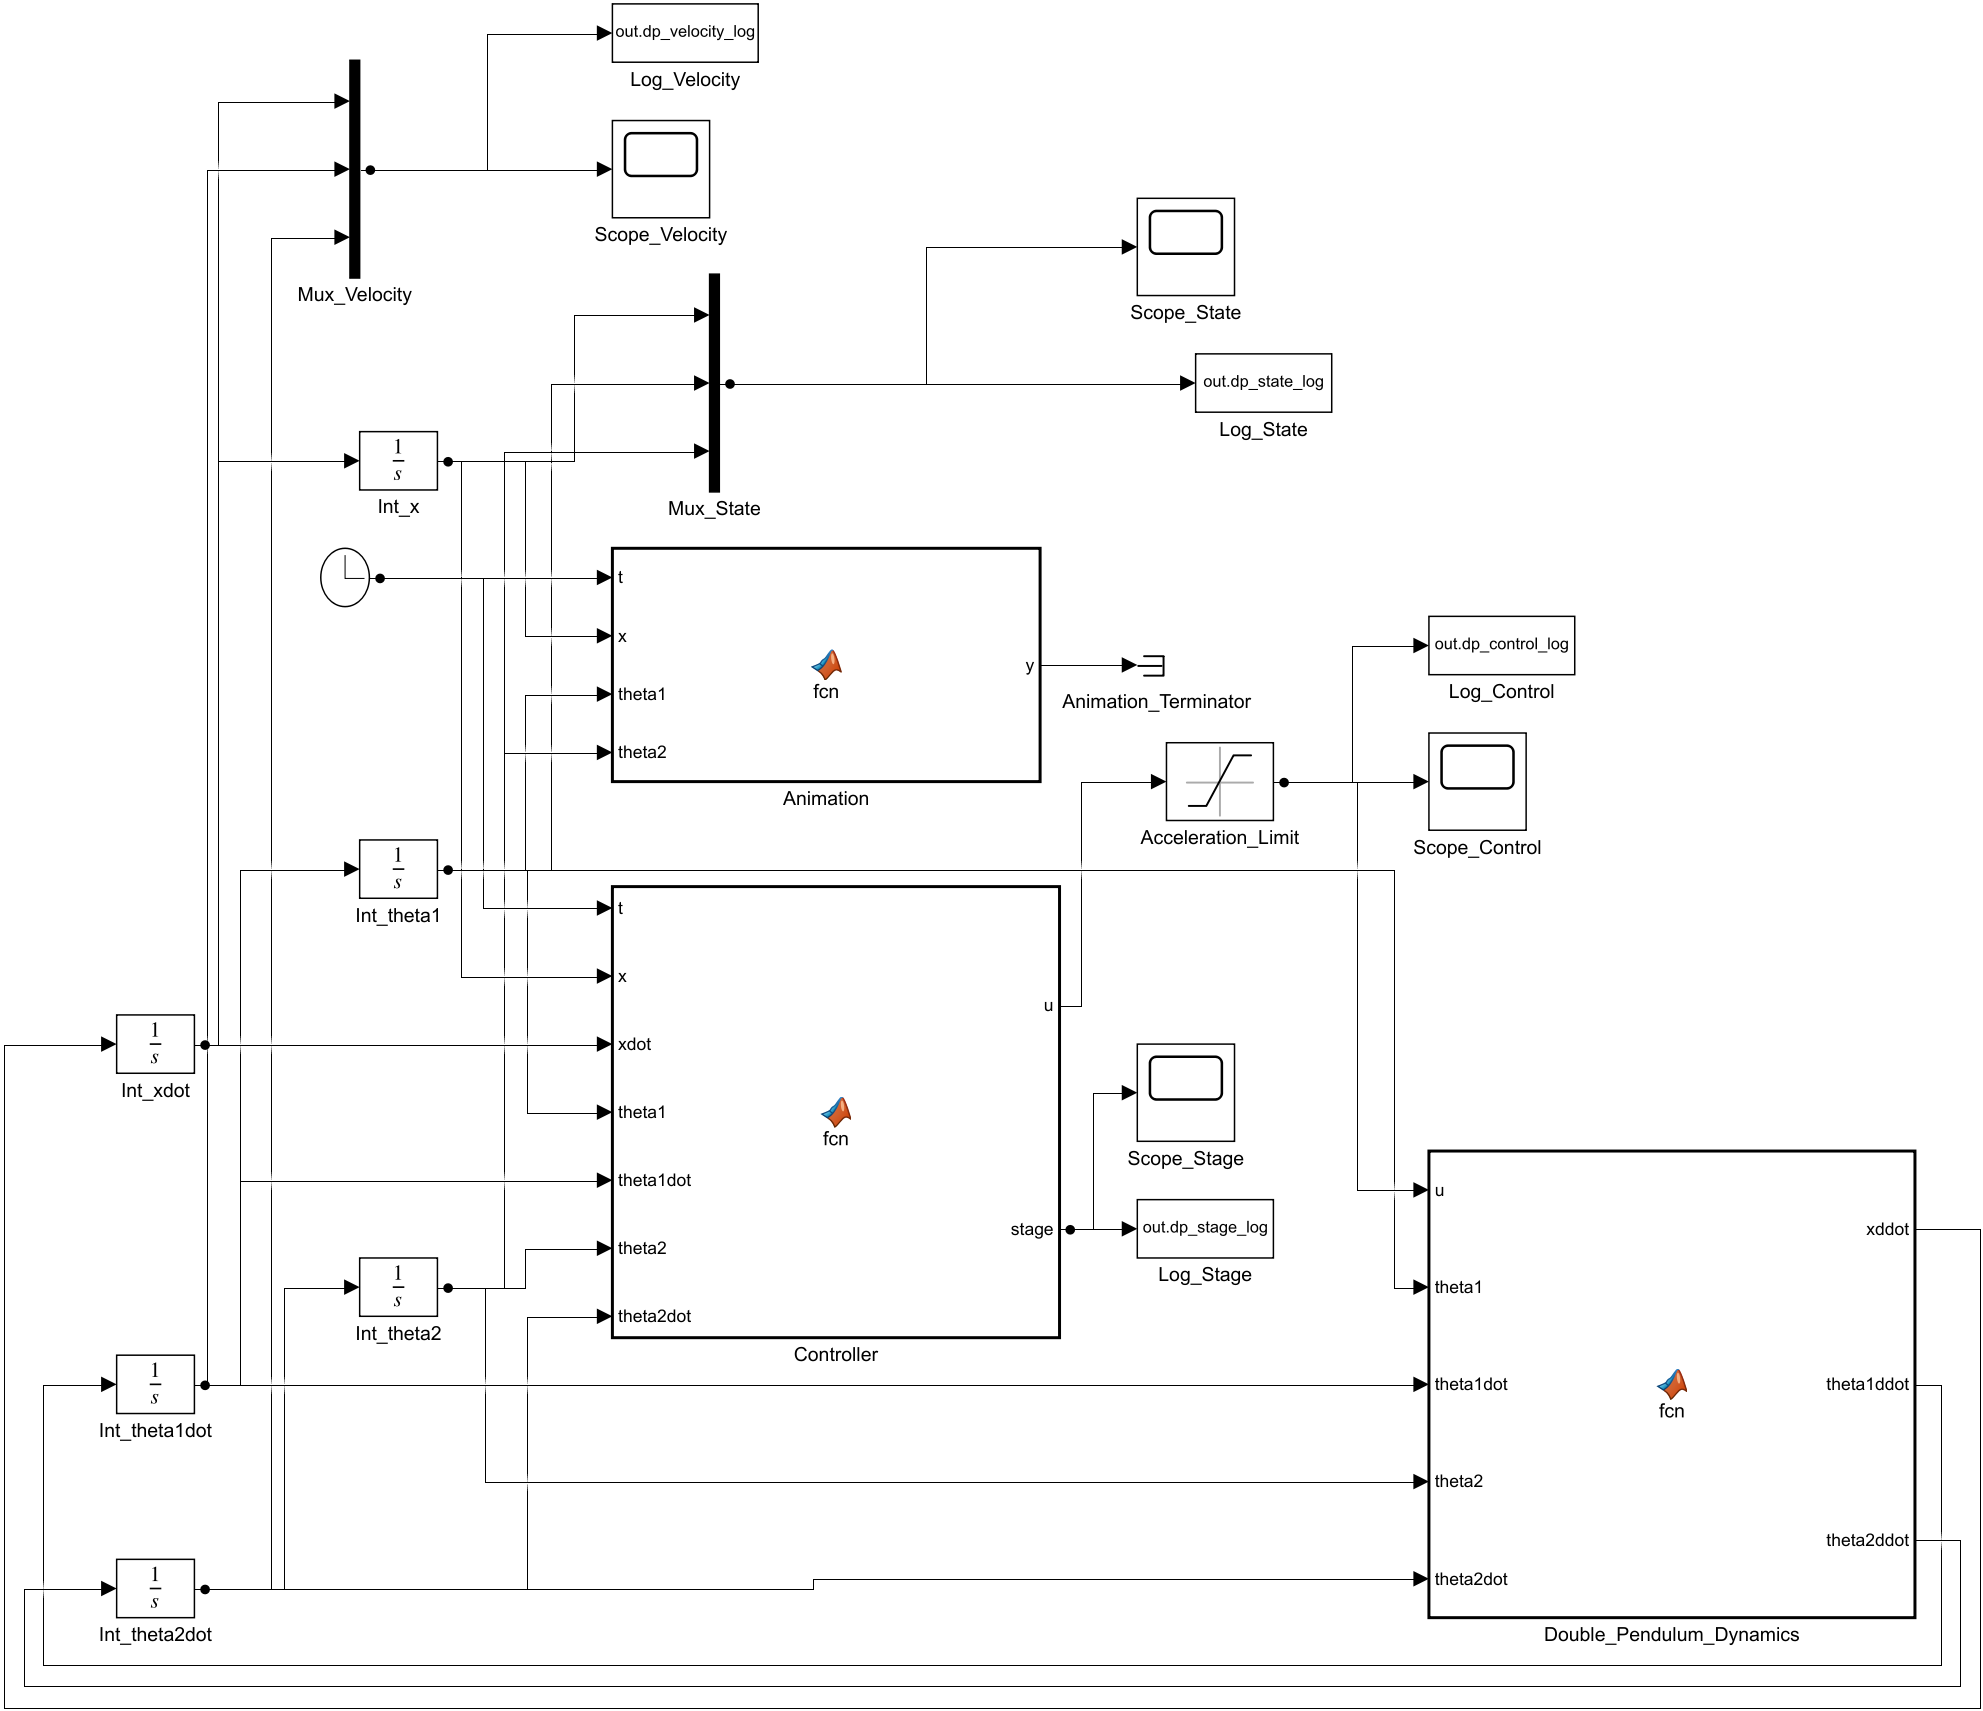
\includegraphics[width=\textwidth]{docs/matlab_simulation_lqr_assets/double_pendulum_balance.png}
        \caption{二级摆直立稳摆模型}
    \end{subfigure}
    \caption{二级摆离线 Simulink 模型}
    \label{fig:dp_models}
\end{figure}

二级状态定义：
\[
    X = [x,\ \theta_1,\ \theta_2,\ \dot{x},\ \dot{\theta}_1,\ \dot{\theta}_2]^{\mathsf T}
\]
两个角度都是相对于竖直向上的绝对角，控制输入 $u$ 为小车加速度。

\subsection{结果示例}

\begin{figure}[htbp]
    \centering
    \begin{subfigure}{0.48\textwidth}
        \centering
        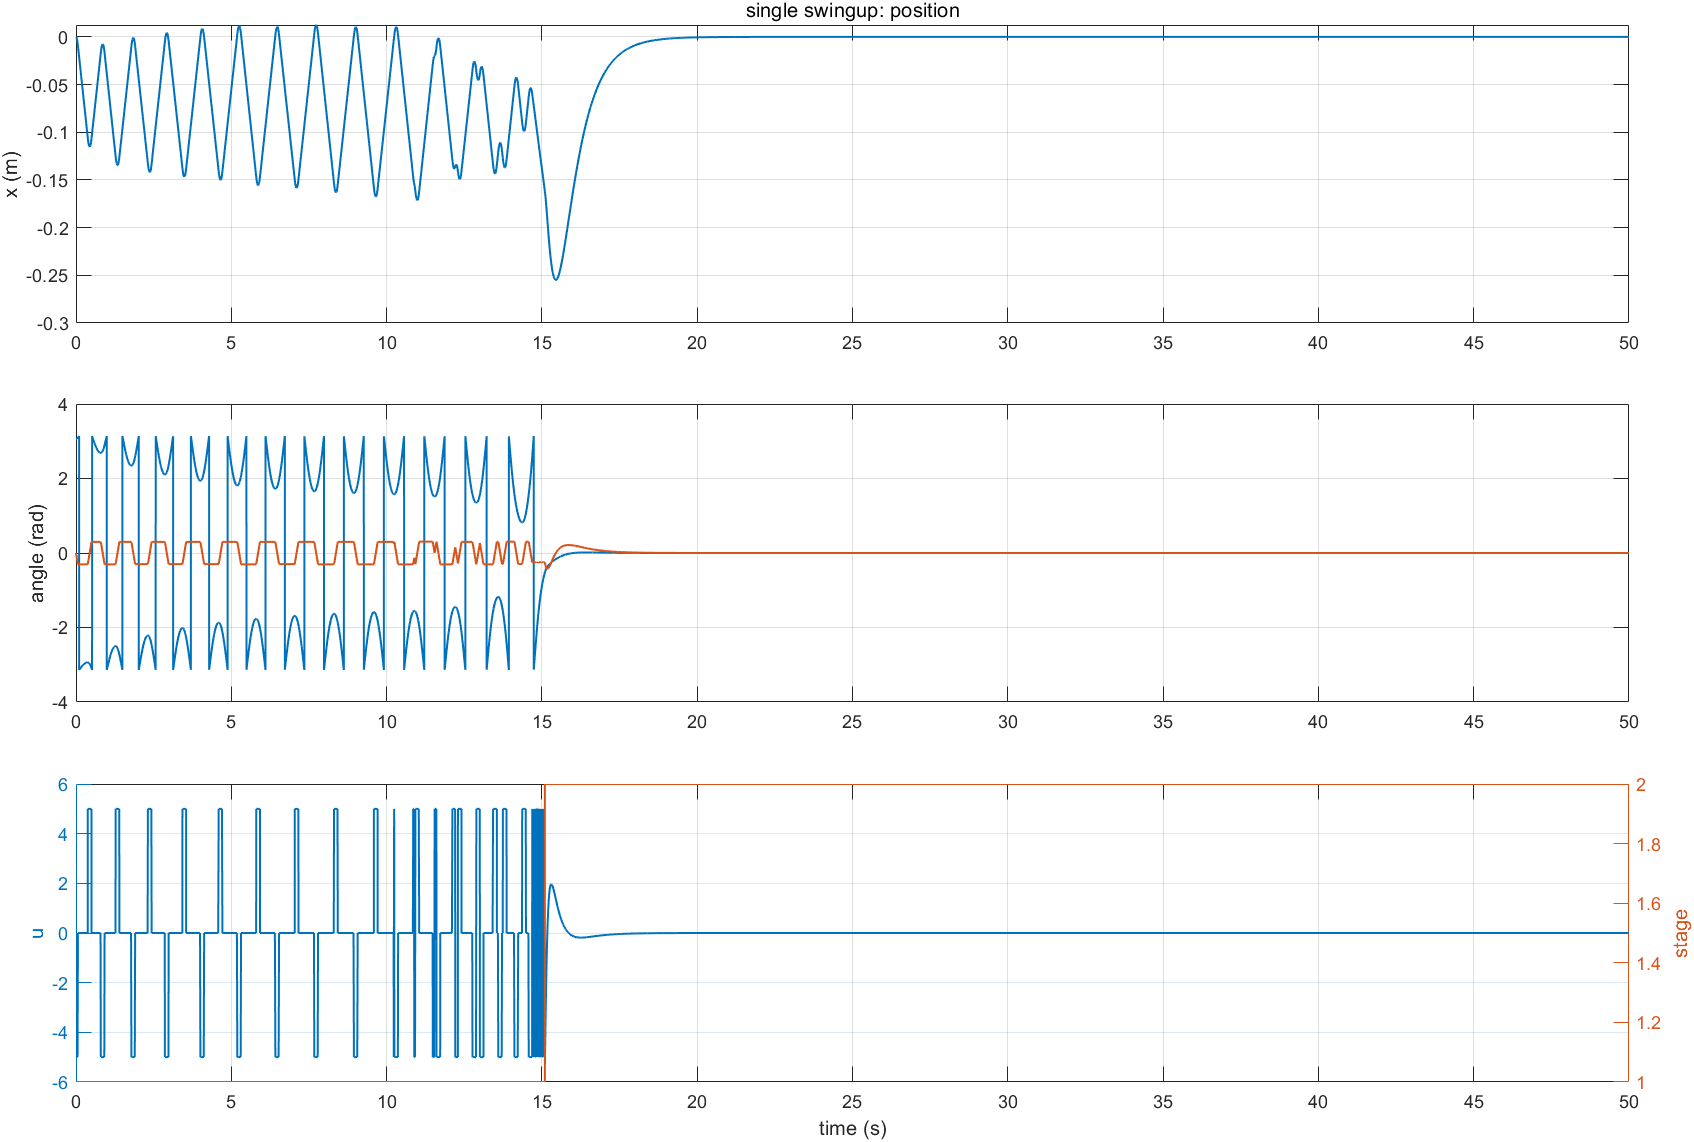
\includegraphics[width=\textwidth]{docs/matlab_simulation_lqr_assets/single_swingup_result.png}
        \caption{一级摆完整摆起结果}
    \end{subfigure}
    \hfill
    \begin{subfigure}{0.48\textwidth}
        \centering
        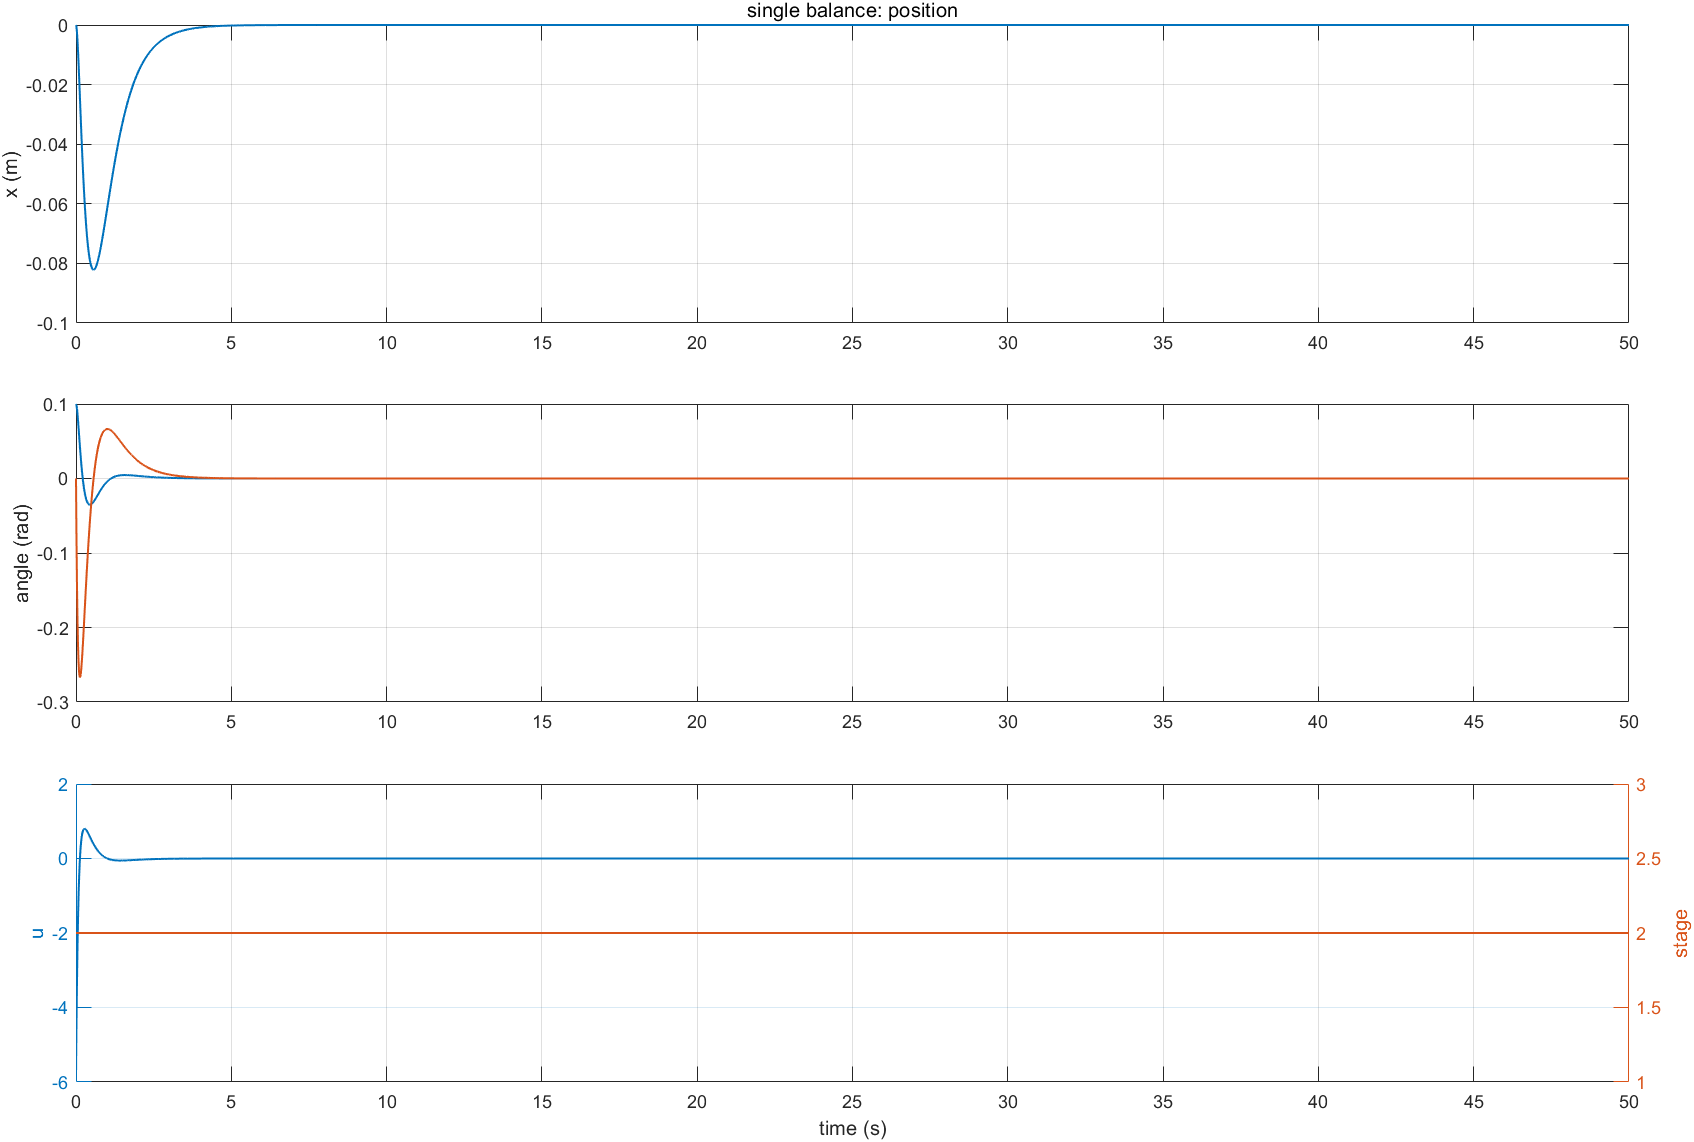
\includegraphics[width=\textwidth]{docs/matlab_simulation_lqr_assets/single_balance_result.png}
        \caption{一级摆稳摆结果}
    \end{subfigure}
    \caption{一级摆离线仿真结果}
    \label{fig:sp_results}
\end{figure}

一级摆起结果图（图~\ref{fig:sp_results} 左）从上到下依次为小车位置、摆角、控制输入与阶段：Stage 从 1 变为 2 后，摆角和小车位置逐渐收敛。稳摆场景（右）从直立附近的小偏差开始，只验证 LQR 的局部稳定性。

\begin{figure}[htbp]
    \centering
    \begin{subfigure}{0.48\textwidth}
        \centering
        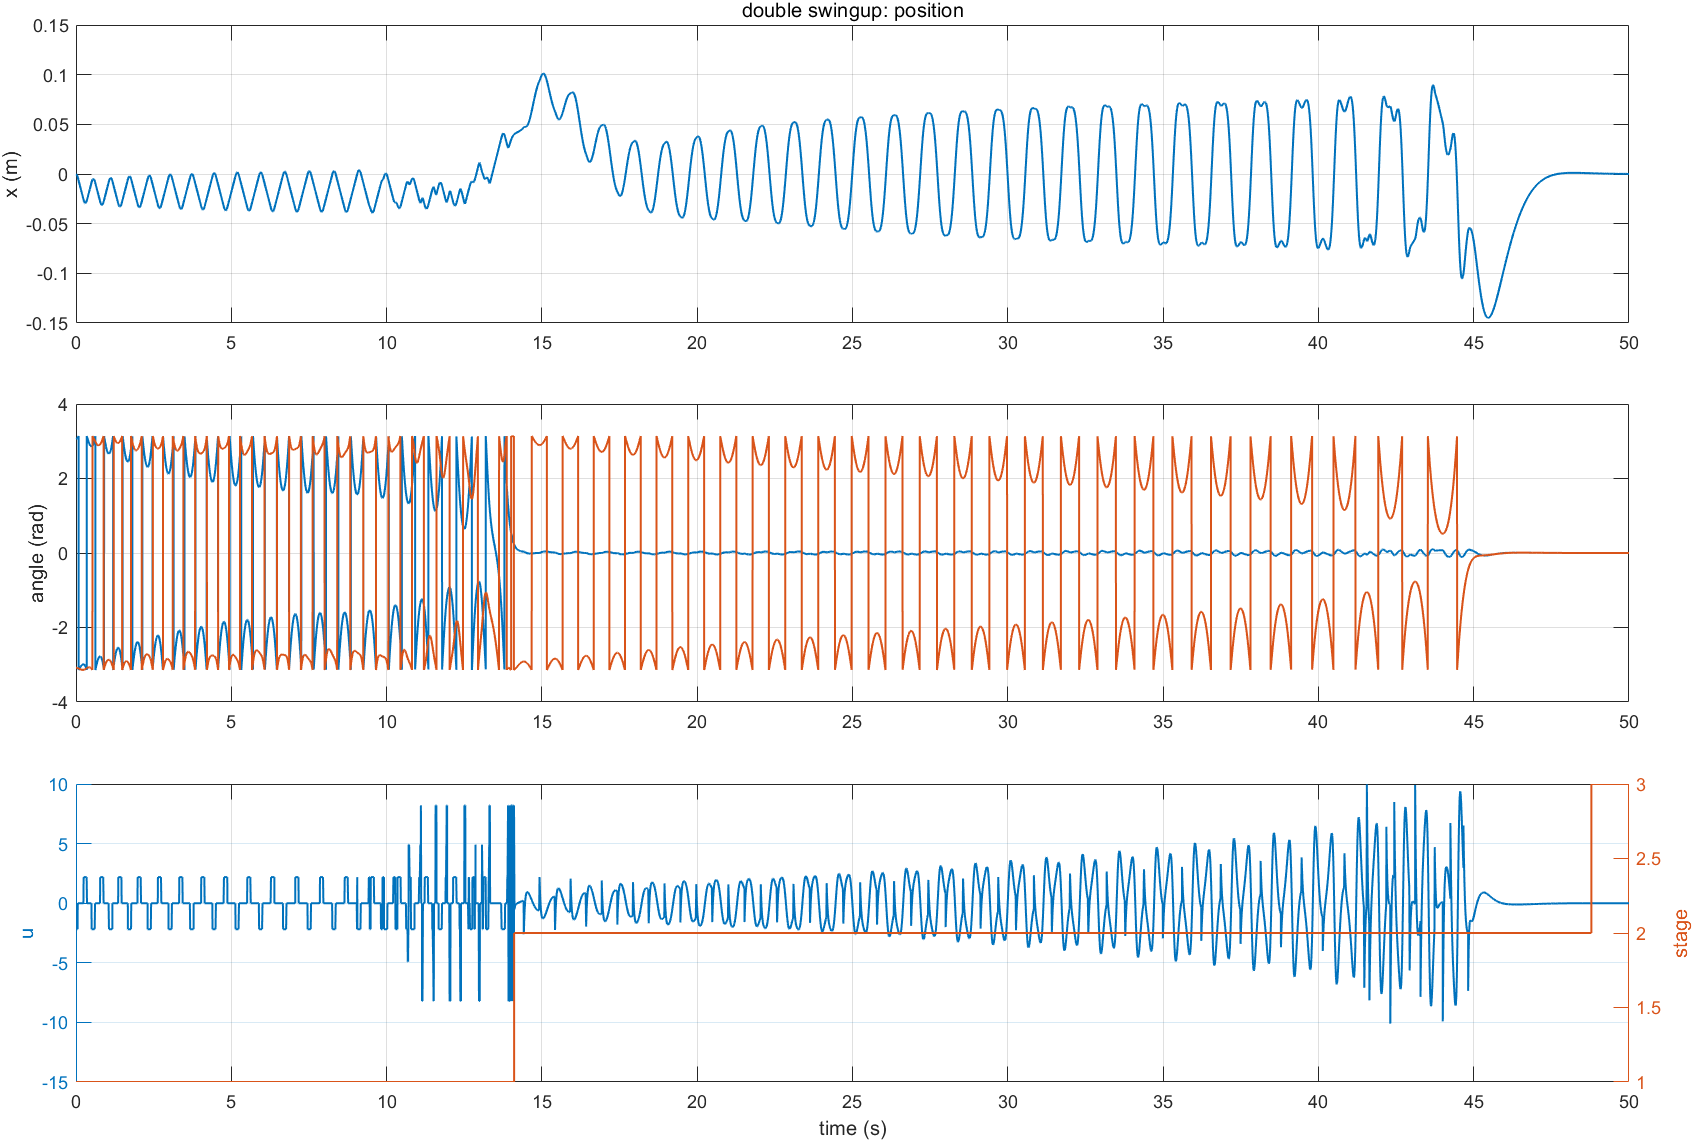
\includegraphics[width=\textwidth]{docs/matlab_simulation_lqr_assets/double_swingup_result.png}
        \caption{二级摆完整摆起结果}
    \end{subfigure}
    \hfill
    \begin{subfigure}{0.48\textwidth}
        \centering
        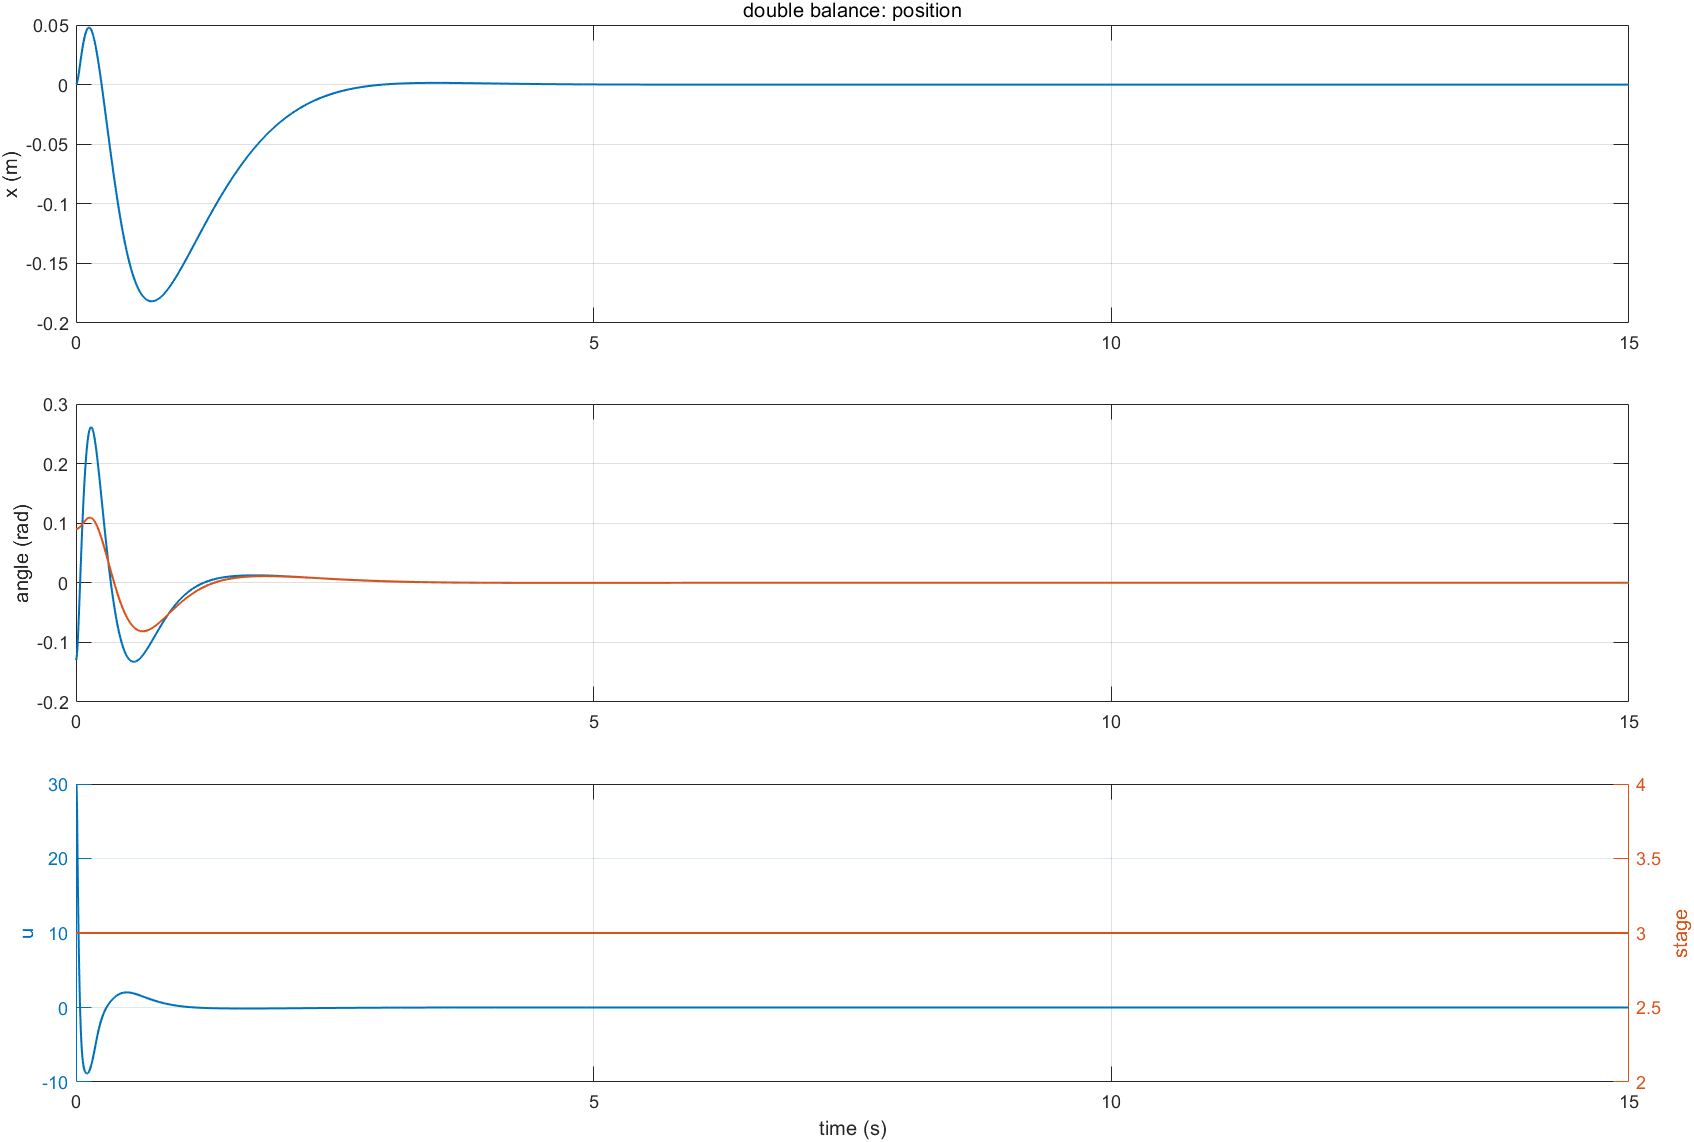
\includegraphics[width=\textwidth]{docs/matlab_simulation_lqr_assets/double_balance_result.png}
        \caption{二级摆稳摆结果}
    \end{subfigure}
    \caption{二级摆离线仿真结果}
    \label{fig:dp_results}
\end{figure}

二级完整摆起结果应访问 Stage 1、2、3，最终两根摆杆角度收敛到 0 附近，同时小车不越过轨道限制（图~\ref{fig:dp_results} 左）。稳摆场景直接从小角度偏差开始，主要用于比较不同 LQR 增益的收敛、轨道占用和控制强度（右）。

\subsection{结果判定与通过条件}

\begin{center}
    \renewcommand{\arraystretch}{1.4}
    \begin{tabular}{@{}l p{10.6cm}@{}}
        \toprule
        \textbf{字段} & \textbf{含义} \\
        \midrule
        \texttt{t} & 时间序列 \\
        \texttt{X} & 状态轨迹 \\
        \texttt{u} & 控制输入 \\
        \texttt{stage} & 控制阶段 \\
        \texttt{passed} & 是否满足全部判据 \\
        \texttt{settled} & 末尾窗口是否收敛 \\
        \texttt{max\_abs\_x} & 最大轨道位移 \\
        \texttt{max\_abs\_u} & 最大控制输入 \\
        \texttt{failed/reason} & 是否提前失败及原因 \\
        \texttt{stages\_visited} & 实际访问的阶段 \\
        \texttt{output\_file} & 本次可复现结果文件 \\
        \bottomrule
    \end{tabular}
\end{center}

摆起场景除收敛、行程和限幅外，还要求访问全部必要阶段：一级为 $[1\ 2]$，二级为 $[1\ 2\ 3]$。

无界面自动验证全部场景：

\begin{lstlisting}[language=Matlab, caption={指定 Simulink 引擎与自动验证}, label={lst:verify}]
r = run_pendulum('double','balance',struct( ...
    'engine','simulink','show_ui',true));

report = verify_pendulum();                  % numeric scenarios only
assert(all([report.passed]));

report = verify_pendulum({'numeric','simulink'});   % both engines
\end{lstlisting}

\subsection{修改算法后的验证顺序}

\begin{center}
    \renewcommand{\arraystretch}{1.3}
    \begin{tabular}{@{}c@{}}
        修改参数或算法 \\
        $\downarrow$ \\
        单场景 \texttt{numeric} 快速测试 \\
        $\downarrow$ \\
        \texttt{balance} 多初值测试 \\
        $\downarrow$ \\
        \texttt{swingup} 完整阶段测试 \\
        $\downarrow$ \\
        \texttt{verify\_pendulum} 全场景测试 \\
        $\downarrow$ \\
        Simulink 引擎对照 \\
        $\downarrow$ \\
        只读实机输入验证 \\
        $\downarrow$ \\
        有限时间实机测试 \\
    \end{tabular}
\end{center}

\begin{lstlisting}[language=Matlab, caption={修改算法后的推荐离线验证命令}, label={lst:verifyseq}]
r1 = run_pendulum('single','balance',struct('engine','numeric','show_ui',false));
r2 = run_pendulum('single','swingup',struct('engine','numeric','show_ui',false));
r3 = run_pendulum('double','balance',struct('engine','numeric','show_ui',false));
r4 = run_pendulum('double','swingup',struct('engine','numeric','show_ui',false));
assert(all([r1.passed r2.passed r3.passed r4.passed]));
\end{lstlisting}

% ======================================================================
\section{控制算法原理}
\label{sec:algorithm}

本节用通俗语言介绍平台的核心控制算法，帮助使用者理解各部分的作用，从而知道「改哪个模块、会产生什么影响」。

\subsection{能量摆起：把下垂的摆杆摇起来}

摆杆初始下垂时，LQR 这类针对直立平衡点设计的线性控制器无法直接起作用，需要先把摆杆「摇」到直立附近。能量摆起的基本思想是：

\begin{itemize}
    \item 比较摆杆当前能量与\textbf{直立位置势能}：能量不足时，让小车沿摆杆运动方向加速，向摆杆泵入能量；
    \item 摆杆像秋千一样越摆越高，振幅不断增大；
    \item 当摆角与角速度同时进入预设的\textbf{捕获窗口}时，切换到 LQR 稳定控制，把摆杆「接住」并稳定在直立位置。
\end{itemize}

能量摆起对摆动方向有要求，一般还需限制小车速度，防止摆起过程中小车撞向轨道两端。二级摆的摆起更复杂：先摆起第一根杆，再保持第一根杆的同时激励第二根杆（三级摆起，见下文）。

\subsection{LQR 稳定：直立附近的反馈控制}

摆杆进入直立邻域后，系统可以用线性模型近似。对线性系统
\[
    \dot{X} = AX + Bu
\]
LQR 选择反馈增益 $K$，使控制律
\[
    u = -KX
\]
最小化性能指标：
\[
    J = \int_{0}^{\infty} \bigl( X^{\mathsf T} Q X + u^{\mathsf T} R u \bigr)\, dt
\]

\begin{itemize}
    \item 增大 $Q(i,i)$：更强地惩罚第 $i$ 个状态偏差，该状态收敛更「硬」；
    \item 增大 $R$：更强地惩罚控制输入，控制通常更温和；
    \item $Q$ 和 $R$ 不是物理参数，而是\textbf{性能权重}，需要结合仿真调参。
\end{itemize}

\subsection{一级摆控制策略}

一级摆只有两个阶段：

\begin{center}
    \renewcommand{\arraystretch}{1.4}
    \begin{tabular}{@{}c l@{}}
        \toprule
        \textbf{Stage} & \textbf{控制方式} \\
        \midrule
        1 & 能量摆起 \\
        2 & LQR 稳摆 \\
        \bottomrule
    \end{tabular}
\end{center}

直立附近的 LQR 控制律为 $u = -KX$，当前增益：
\[
    K = \begin{bmatrix} -10 & 58.6 & -12.23 & 10.69 \end{bmatrix}
\]
即（实机 Simulink 中的写法）：
\[
    u = 10\,x - 58.6\,\theta_1 + 12.23\,\dot{x} - 10.69\,\dot{\theta}_1
\]
加速度指令限幅 $[-10,10]\,\text{m/s}^2$。离直立较远时采用能量摆起，通过摆杆能量误差决定小车加速度方向，并限制小车速度；进入捕获角度和角速度窗口后切换到 LQR。

\subsection{二级摆三阶段控制}

\begin{table}[htbp]
    \centering
    \caption{二级摆三阶段控制策略}
    \label{tab:stages2}
    \renewcommand{\arraystretch}{1.4}
    \begin{tabular}{@{}c p{4.6cm} p{7.2cm}@{}}
        \toprule
        \textbf{Stage} & \textbf{目标} & \textbf{主要控制方式} \\
        \midrule
        1 & 摆起第一根杆 & 一级摆能量控制 \\
        2 & 保持第一根杆并摆起第二根杆 & 一级杆 LQR + 第二杆能量泵入 \\
        3 & 两根杆直立稳定 & 六状态 LQR \\
        \bottomrule
    \end{tabular}
\end{table}

Stage 2 接近捕获区域时会提前引入六状态反馈。若从 Stage 3 跌出稳定范围，控制器会根据角度回退到 Stage 1 或 Stage 2。二级 LQR 控制律为 $u = -KX$，状态顺序为
\[
    [x,\ \theta_1,\ \theta_2,\ \dot{x},\ \dot{\theta}_1,\ \dot{\theta}_2]
\]
当前增益见表~\ref{tab:K2}，加速度限幅 $[-30,30]\,\text{m/s}^2$。

与该增益对应的当前权重参数来自 \texttt{matlab/double\_pendulum/dp\_best\_lqr.m}：
\[
Q=\operatorname{diag}\!\left(
192.8017030460,
34.3800101639,
801.9896042159,
24.9635933446,
7.3464894226,
4.3552741723
\right),
\qquad
R=0.4475475561.
\]
这些数值是当前已保存控制器的复现参数；后文代码中的 $Q=\operatorname{diag}(200,40,800,25,8,5)$、$R=0.45$ 是便于重新设计的近似示例，不应误认为与表~\ref{tab:K2} 完全对应。

\begin{table}[htbp]
    \centering
    \caption{二级摆当前 LQR 增益（$u = -KX$）}
    \label{tab:K2}
    \renewcommand{\arraystretch}{1.35}
    \begin{tabular}{@{}l l@{}}
        \toprule
        \textbf{状态} & \textbf{增益} \\
        \midrule
        $x$ & 20.755626070279462 \\
        $\theta_1$ & 136.68455751706179 \\
        $\theta_2$ & $-254.85837173801795$ \\
        $\dot{x}$ & 24.440647335478328 \\
        $\dot{\theta}_1$ & 3.3044801353394511 \\
        $\dot{\theta}_2$ & $-40.750449384516202$ \\
        \bottomrule
    \end{tabular}
\end{table}

\begin{dangerbox}
    \textbf{状态顺序必须严格保持。} 一级为 $[x,\ \theta_1,\ \dot{x},\ \dot{\theta}_1]$，二级为 $[x,\ \theta_1,\ \theta_2,\ \dot{x},\ \dot{\theta}_1,\ \dot{\theta}_2]$。替换 LQR Gain 块时如果顺序搞错，会导致控制方向错误甚至发散。
\end{dangerbox}

\subsection{在 MATLAB 中设计新增益}

\begin{lstlisting}[language=Matlab, caption={二级摆 LQR 设计与评估}, label={lst:lqrdesign}]
P = dp_config();
[A,B,info] = dp_linearize(P,true);   % linearize + check controllability rank 6

Q = diag([200 40 800 25 8 5]);
R = 0.45;
L = dp_lqr_design(Q,R,true);
K = L.K;

evaluation = dp_evaluate_controller(K,P);   % nonlinear multi-start test
\end{lstlisting}

\texttt{dp\_linearize} 在直立平衡点 $X=0,\ u=0$ 附近采用中心差分线性化，并检查可控性矩阵秩是否为 6。设计新增益后必须检查：

\begin{itemize}
    \item $L$.poles 的实部全部小于 0（闭环极点稳定）；
    \item 可控性秩等于状态数；
    \item 非线性多初值仿真通过；
    \item 控制输入没有长期饱和；
    \item 小车位置没有超过轨道限制。
\end{itemize}

\texttt{dp\_evaluate\_controller} 会跨多个非线性初始状态评价稳定性、行程、饱和、控制能量和收敛时间，比只看闭环极点可靠。

\begin{tipbox}
    不要直接覆盖 \texttt{dp\_best\_lqr.m}。先保存候选增益、运行全部测试，确认后再更新已知良好增益。
\end{tipbox}

\subsection{自动搜索与优化}

\begin{lstlisting}[language=Matlab, caption={LQR 权重自动搜索（运行时间较长）}, label={lst:search}]
search = dp_lqr_optimize(struct('make_plots',false));
result = dp_optimize_stage2_robust();
\end{lstlisting}

\texttt{dp\_lqr\_optimize} 对 Q 对角元素和 R 进行对数空间采样，调用 \texttt{lqr(A,B,Q,R)} 得到候选 $K$，在多个非线性场景中评价，淘汰不稳定、越轨或输入不合格的结果，并对排名靠前的区域继续细化。\texttt{dp\_optimize\_stage2\_robust} 专门搜索第二杆远区/近区增益、捕获角速度和目标能量，并使用对称初态及执行器非理想配置验证鲁棒性。

\begin{warnbox}
    优化脚本可能运行较长时间，且输出目录可能很大。优化结果\textbf{不会自动替换}项目当前基线增益。
\end{warnbox}

% ======================================================================
\section{从离线仿真迁移到实机}
\label{sec:migration}

离线仿真通过后，把算法搬到实机 Simulink 时\textbf{不能只复制一个 Gain 块}，还需要逐项核对：

\begin{center}
    \renewcommand{\arraystretch}{1.4}
    \begin{tabular}{@{}l p{5.4cm} p{5.6cm}@{}}
        \toprule
        \textbf{项目} & \textbf{离线仿真} & \textbf{实机模型} \\
        \midrule
        输入来源 & 数学动力学 & 编码器计数 \\
        控制输出 & 加速度 & 最终需要转换为电压 \\
        速度 & 理想状态或数值积分 & 编码器差分与滤波 \\
        饱和 & 模型设定 & 驱动器和软件双重限制 \\
        时间 & 确定性数值步长 & 100/200\,Hz 实际调度 \\
        安全 & 越界停止仿真 & 物理限位、软件限位、急停 \\
        \bottomrule
    \end{tabular}
\end{center}

正确的迁移顺序：

\begin{enumerate}
    \item 保持状态定义和符号一致；
    \item 将离线 LQR/摆起输出接到实机的加速度到电压模块；
    \item 保留实机 \texttt{Travel\_and\_faults}；
    \item 保持一级 10\,ms、二级 5\,ms 的离散状态更新；
    \item 使用记录回放比较 MATLAB 离线算法与实机图的逐采样输出；
    \item 先只读，再有限时间、低风险实机测试。
\end{enumerate}

% ======================================================================
\section{实机运行}
\label{sec:hardware}

\subsection{启动命令}

一级摆：
\begin{lstlisting}[language=Matlab, caption={一级摆实机启动}, label={lst:run1}]
start_pendulum_simulink(1)
\end{lstlisting}

二级摆：
\begin{lstlisting}[language=Matlab, caption={二级摆实机启动}, label={lst:run2}]
start_pendulum_simulink(2)
\end{lstlisting}

运行入口会自动执行图~\ref{alg:seq} 所示的完整序列：

\begin{algorithm}[htbp]
    \caption{实机运行自动序列}
    \label{alg:seq}
    \begin{algorithmic}[1]
        \State 只读预检（不打开伺服输出）
        \State 硬件初始化
        \State 自动回中
        \State 下垂零点采集
        \State 启动控制（能量摆起 $\rightarrow$ LQR 稳定）
        \State 持续记录数据
    \end{algorithmic}
\end{algorithm}

\subsection{运行前检查清单}

\begin{itemize}[label=\cmark]
    \item 在电脑、MATLAB/Simulink、板卡、伺服驱动器或任何相关设备重启、复位或重新上电前，急停按钮已经按下；
    \item 重启和软件恢复期间保持急停，只有完成以下全部检查后才由现场操作人员解除；
    \item 轨道无障碍物；
    \item 两侧物理限位可靠；
    \item 急停按钮功能正常并可立即再次按下；
    \item 摆杆和编码器机械连接正常；
    \item 设备型号、通道和方向没有改变；
    \item 通信检查和只读预检通过，控制输出仍处于关闭状态；
    \item 首次测试采用有限运行时间并有人值守。
\end{itemize}

\subsection{首次有限时间测试}

首次实机测试建议使用有限运行时间：

\begin{lstlisting}[language=Matlab, caption={有限时间首次测试（10 秒）}, label={lst:firstrun}]
start_pendulum_simulink(1,'hardware',10);
start_pendulum_simulink(2,'hardware',10);
\end{lstlisting}

\subsection{停止运行}

点击 Simulink Stop 或按 \texttt{Ctrl+C} 停止运行时，硬件会话的结束逻辑负责关闭输出。

\begin{warnbox}
    不要使用任务管理器强制终止 MATLAB 作为常规停止方式。
\end{warnbox}

\subsection{运行前离线验证}

在项目根目录打开 MATLAB，验证用户保存的 \texttt{.slx}（不会重建模型）：

\begin{lstlisting}[language=Matlab, caption={实机模型离线验证与只读模式}, label={lst:pnverify}]
addpath('matlab/native_simulink');
report = pn_verify();          % verify the saved .slx, no rebuild
assert(report.passed);
\end{lstlisting}

该测试不会打开物理硬件，会检查：模型能够更新和执行；控制器仍使用标准 Simulink 块；一级和二级各阶段均被覆盖；软件行程恢复被触发；输出与项目当前 MATLAB 参考递推一致。

\begin{warnbox}
    如果算法被有意替换，旧参考递推不再适用，差分测试会失败。这时应同步建立新算法的独立参考计算，而不是简单删除断言。
\end{warnbox}

同一个测试还会检查左右限位、双限位、软件行程、超大加速度及 \texttt{NaN/Inf} 命令，确认硬件层独立将电压置零并报告故障。

只读硬件检查（读取真实输入并运行控制图，但不打开伺服输出）：

\begin{lstlisting}[language=Matlab, caption={只读硬件检查}, label={lst:readonly}]
start_pendulum_simulink(1,'readonly',5);  % order 1
start_pendulum_simulink(2,'readonly',5);  % order 2
\end{lstlisting}

% ======================================================================
\section{安全规范}
\label{sec:safety}

\begin{dangerbox}
    \textbf{重启必须急停：}只要电脑或任何相关设备需要重启，必须在重启前按下急停按钮，并在重启和软件恢复全过程保持急停。该要求同样适用于 MATLAB/Simulink 重启、板卡复位、伺服驱动器重启、系统断电后重新上电、驱动报警复位和程序异常退出。完成轨道清障、人员撤离、限位检查、通信检查和只读预检后，才允许现场人员解除急停。
\end{dangerbox}

\subsection{安全边界设计}

平台的安全边界由 \texttt{Travel\_and\_faults} 模块与硬件层共同构成（见第~\ref{sec:simulink} 节）：

\begin{itemize}
    \item 一级摆：到达预警位置且控制仍指向外侧时输出置零，并清除积分器；
    \item 二级摆：到达预警位置且控制仍指向外侧时施加 0.03\,V 向中心恢复电压并清除积分状态；
    \item 物理限位、软件停止位置、非有限数值（\texttt{NaN/Inf}）任一触发，立即输出 0\,V 并置 \texttt{Fault}=1；
    \item 停止运行时硬件层负责关闭输出。
\end{itemize}

\subsection{禁止修改区域}

\begin{dangerbox}
    算法使用者不应修改以下内容：
    \begin{itemize}[nosep]
        \item \texttt{Hardware} 内的 S-Function 名称、端口和反馈路径；
        \item \texttt{pn\_io\_sfun.m} 的采集/写入时序；
        \item \texttt{PnHardwareSession.m} 的安全停机逻辑；
        \item \texttt{Real-Time Sync} 的采样周期和同步配置；
        \item 顶层五路测量/状态信号和一路加速度反馈线；
        \item \texttt{Travel\_and\_faults} 中的物理限位停机路径；
        \item 电压上限、软件停止位置或机械行程限制，除非经过新的硬件安全评审。
    \end{itemize}
\end{dangerbox}

\begin{tipbox}
    如果新算法需要额外参数，优先在 \texttt{Control} 内使用 Constant、Gain 或 Data Store，而不是增加顶层硬件端口。
\end{tipbox}

\subsection{故障处理原则}

\begin{itemize}
    \item 实机启动失败时，检查只读预检结果、设备连接、限位状态、回中过程和零点稳定性；
    \item \textbf{不要通过删除 Fault 或扩大安全范围来绕过失败}；
    \item 控制方向相反时，先检查算法使用的状态符号和反馈增益顺序，不要直接交换硬件通道或修改顶层接线（那样会同时破坏回中和安全方向定义）；
    \item 一开始就产生很大电压时，检查离散状态初值、第一帧差分、积分器初值、角度零点以及输出限幅——状态估计应在首帧用当前测量初始化。
    \item 电脑、控制软件、板卡或驱动器发生重启、掉电恢复或异常退出后，不得直接继续实验；先按下急停，再从运行前检查和只读预检重新开始。
\end{itemize}

% ======================================================================
\section{常见问题排查}
\label{sec:faq}

\begin{itemize}

    \item \textbf{修改保存后又恢复成旧算法}： 原因通常是运行了 \texttt{pn\_build()} 或 \texttt{pn\_verify(true)}。默认的 \texttt{pn\_verify()} 不会重建模型。

    \item \textbf{模型可以仿真，但实机启动失败}： 检查只读预检结果、设备连接、限位状态、回中过程和零点稳定性。不要通过删除 Fault 或扩大安全范围来绕过失败。

    \item \textbf{控制方向相反}： 先检查算法使用的状态符号和反馈增益顺序。不要直接交换硬件通道或修改顶层接线，因为这样会同时破坏回中和安全方向定义。

    \item \textbf{一开始就产生很大电压}： 检查离散状态初值、第一帧差分、积分器初值、角度零点以及输出限幅。状态估计应在首帧用当前测量初始化。

    \item \textbf{二级摆无法进入 Stage 3}： 检查 \texttt{Stage\_supervisor} 的角度、角速度、小车速度和运动方向条件；手动扶正时两根摆杆都必须进入捕获窗口。

    \item \textbf{自定义算法验证失败}： \texttt{pn\_verify()} 的数值回归针对内置算法。替换算法后应建立自己的效果测试，同时保持五入一出接口和硬件保护不变。

    \item \textbf{LQR 极点稳定，但非线性仿真失败}： LQR 只保证平衡点附近线性模型的局部性质。应减小初始偏差、检查饱和，或改进摆起到 LQR 的捕获条件。

    \item \textbf{调大 Q 后反而越轨或振荡}： 更大的状态惩罚可能产生更激烈的控制，触发输入饱和并破坏线性设计假设。必须同时查看控制输入 $u$ 和小车位置 $x$。

    \item \textbf{数值仿真通过，Simulink 不一致}： 检查固定步长、离散控制采样、零阶保持、状态顺序和初值。二级摆起控制器含阶段记忆，开始新仿真前必须正确重置。

    \item \textbf{完整摆起没有进入 Stage 3}： 检查捕获角度、角速度、小车速度和方向条件，而不是只增大摆起增益。

    \item \textbf{修改生成的 SLX 后再次运行又被覆盖}： 一级 \texttt{sp\_build\_model.m} 和二级 \texttt{build\_model.m} 是离线模型的生成源；实机模型则由 \texttt{pn\_build.m} 生成。需要永久修改内置结构时同步更新生成脚本。

\end{itemize}

\newpage
\appendix

% ======================================================================
\section{附录 A：常用命令速查}

\begin{longtable}{@{}p{8.0cm} p{6.4cm}@{}}
    \caption{PendulumLab 常用命令速查表} \label{tab:commands} \\
    \toprule
    \textbf{命令} & \textbf{用途} \\
    \midrule
    \endfirsthead
    \toprule
    \textbf{命令} & \textbf{用途} \\
    \midrule
    \endhead
    \bottomrule
    \endlastfoot
    \seqsplit{\texttt{addpath('matlab'); setup\_pendulum;}} & 初始化离线仿真路径 \\
    \seqsplit{\texttt{run\_pendulum('single','swingup')}} & 一级摆完整摆起仿真 \\
    \seqsplit{\texttt{run\_pendulum('single','balance')}} & 一级摆直立稳摆仿真 \\
    \seqsplit{\texttt{run\_pendulum('double','swingup')}} & 二级摆完整摆起仿真 \\
    \seqsplit{\texttt{run\_pendulum('double','balance')}} & 二级摆直立稳摆仿真 \\
    \seqsplit{\texttt{run\_pendulum('double','balance', struct('engine','simulink','show\_ui',true))}} & 使用 Simulink 引擎并显示界面 \\
    \seqsplit{\texttt{verify\_pendulum()}} & 无界面自动验证全部数值场景 \\
    \seqsplit{\texttt{verify\_pendulum(\{'numeric','simulink'\}})} & 同时验证数值与 Simulink 引擎 \\
    \seqsplit{\texttt{dp\_lqr\_design(Q,R,true)}} & 由 Q、R 设计二级 LQR 增益 \\
    \seqsplit{\texttt{dp\_evaluate\_controller(K,P)}} & 多初值非线性评估候选增益 \\
    \seqsplit{\texttt{dp\_lqr\_optimize(...)}} & 自动搜索 LQR 权重（耗时） \\
    \seqsplit{\texttt{addpath('matlab/native\_simulink')}} & 加入实机模型路径 \\
    \seqsplit{\texttt{pn\_verify(false)}} & 验证用户保存的 \seqsplit{\texttt{.slx}}（不重建） \\
    \seqsplit{\texttt{pn\_verify\_faults()}} & 故障输出测试（不打开实机） \\
    \seqsplit{\texttt{start\_pendulum\_simulink(1,'readonly',5)}} & 一级摆只读运行 5\,s \\
    \seqsplit{\texttt{start\_pendulum\_simulink(2,'readonly',5)}} & 二级摆只读运行 5\,s \\
    \seqsplit{\texttt{start\_pendulum\_simulink(1)}} & 一级摆实机运行 \\
    \seqsplit{\texttt{start\_pendulum\_simulink(2)}} & 二级摆实机运行 \\
    \seqsplit{\texttt{start\_pendulum\_simulink(1,'hardware',10)}} & 一级摆有限时间首次测试（10\,s） \\
\end{longtable}

% ======================================================================
\section{附录 B：文件地图与修改建议}

修改算法时，从下表找到对应的优先修改文件：

\begin{center}
    \renewcommand{\arraystretch}{1.4}
    \begin{tabular}{@{}p{5.6cm} p{6.2cm} p{3.6cm}@{}}
        \toprule
        \textbf{目标} & \textbf{优先修改文件} & \textbf{说明} \\
        \midrule
        一级物理参数 & \texttt{sp\_config.m} & 参数、初值、阈值 \\
        一级摆起/LQR & \texttt{sp\_control.m} & 能量摆起与切换逻辑 \\
        一级动力学 & \texttt{sp\_dynamics.m} & 非线性动力学方程 \\
        二级物理参数和阈值 & \texttt{dp\_config.m} & 参数、非理想因素、限幅 \\
        二级场景初值 & \texttt{dp\_scenario\_config.m} & 摆起/稳摆初值与时长 \\
        二级三级摆起 & \texttt{dp\_swingup\_control.m} & 摆起、捕获、LQR、轨道制动 \\
        二级 LQR 设计 & \texttt{dp\_lqr\_design.m} & 由 Q、R 生成增益 \\
        二级当前基线增益 & \texttt{dp\_best\_lqr.m} & \textbf{仅在验证后更新} \\
        离线 Simulink 结构 & \texttt{sp\_build\_model.m} 或 \texttt{build\_model.m} & 生成离线模型 \\
        实机控制算法 & 直接修改 \texttt{Control} 内部并保存 \texttt{.slx} & 保持 5 入 1 出接口 \\
        \bottomrule
    \end{tabular}
\end{center}

\begin{warnbox}
    修改前保留已知良好参数；修改后保存运行结果、参数、MATLAB 版本和通过指标，确保实验能够复现。
\end{warnbox}

\vfill
\begin{center}
    {\color{gray!60}\rule{0.4\textwidth}{0.4pt}} \\[1em]
    {\small\color{gray} PendulumLab 实验平台 · 文档版本 V2.0 · \today} \\[0.6em]
    {\color{gray} --- 文档结束 ---}
\end{center}

\end{document}
